%% Le lingue utilizzate, che verranno passate come opzioni al pacchetto babel. Come sempre, l'ultima indicata sarà quella primaria.
%% Se si utilizzano una o più lingue diverse da "italian" o "english", leggere le istruzioni in fondo.
\def\thudbabelopt{english,italian}
%% Valori ammessi per target: bach (tesi triennale), mst (tesi magistrale), phd (tesi di dottorato).
%% Valori ammessi per aauheader: '' (vuoto -> nessun header Alpen Adria Univeristat), aics (Department of Artificial Intelligence and Cybersecurity), informatics (Department of Informatics Systems). Il nome del dipartimento è allineato con la versione inglese del logo UniUD.
%% Valori ammessi per style: '' (vuoto -> stile moderno), old (stile tradizionale).
\documentclass[target=bach,aauheader=,style=]{thud}

%% --- Informazioni sulla tesi ---
%% Per tutti i tipi di tesi
% Scommentare quello di interesse, o mettete quello che vi pare
\course{Informatica}
%\course{Internet of Things, Big Data e Web}
%\course{Matematica}
%\course{Comunicazione Multimediale e Tecnologie dell'Informazione}
\title{Comparazione sperimentale \\ di algoritmi di cifratura lightweight \\ su microcontrollori embedded}
\author{Jacopo Plozner}
\supervisor{Prof.\ Marino Miculan}
%\cosupervisor{Arch.\ Rambaldo Melandri \and Dott.\ Giorgio Perozzi}
\tutor{Dott.\ Paolo Casoto}
%% Campi obbligatori: \title, \author e \course.
%% Altri campi disponibili: \reviewer, \tutor, \chair, \date (anno accademico, calcolato in automatico), \rights
%% Con \supervisor, \cosupervisor, \reviewer e \tutor si possono indicare più nomi separati da \and.
%% Per le sole tesi di dottorato:
%\phdnumber{313}
%\cycle{XXVIII}
%\contacts{Via della Sintassi Astratta, 0/1\\65536 Gigatera --- Italia\\+39 0123 456789\\\texttt{http://www.example.com}\\\texttt{inbox@example.com}}

%% --- Pacchetti consigliati ---
%% pdfx: per generare il PDF/A per l'archiviazione. Necessario solo per la versione finale
\usepackage[a-1b]{pdfx}
%% hyperref: Regola le impostazioni della creazione del PDF... più tante altre cose. Ricordarsi di usare l'opzione pdfa.
\usepackage[pdfa]{hyperref}
%% tocbibind: Inserisce nell'indice anche la lista delle figure, la bibliografia, ecc.

%% --- Stili di pagina disponibili (comando \pagestyle) ---
%% sfbig (predefinito): Apertura delle parti e dei capitoli col numero grande; titoli delle parti e dei capitoli e intestazioni di pagina in sans serif.
%% big: Come "sfbig", solo serif.
%% plain: Apertura delle parti e dei capitoli tradizionali di LaTeX; intestazioni di pagina come "big".
\usepackage{float} % figure EXACTLY here
\usepackage{MnSymbol} % simboli
\usepackage{algorithm} % algoritmi
\usepackage{algpseudocode} % pseudocodice

\usepackage{tabularx} %multicolonne

\usepackage{multirow} %multitighe

\usepackage{tikz} % crypto figures
\usetikzlibrary{calc}
\usetikzlibrary{crypto.symbols}
\usetikzlibrary {positioning}
\usetikzlibrary{shapes}
\tikzset{sparsam/.style={inner sep=1pt}}
\tikzset{bitwidth/.style={above=-1pt, font=\tiny}}
\tikzset{next/.style={->, >=latex}}

\usepackage[dvipsnames]{xcolor} % colori
\definecolor{mGreen}{rgb}{0,0.6,0}
\definecolor{mGray}{rgb}{0.5,0.5,0.5}
\definecolor{mPurple}{rgb}{0.58,0,0.82}
\definecolor{backgroundColour}{rgb}{0.95,0.95,0.92}

\usepackage{listings} % codice C
\lstdefinestyle{CStyle}{
	backgroundcolor=\color{backgroundColour},   
	commentstyle=\color{mGreen},
	keywordstyle=\color{magenta},
	numberstyle=\tiny\color{mGray},
	stringstyle=\color{mPurple},
	basicstyle=\footnotesize,
	breakatwhitespace=false,         
	breaklines=true,                 
	captionpos=b,                    
	keepspaces=true,                 
	numbers=left,                    
	numbersep=5pt,                  
	showspaces=false,                
	showstringspaces=false,
	showtabs=false,                  
	tabsize=2,
	language=C
}

\begin{document}
\maketitle

%% Dedica (opzionale)
\begin{dedication}
	A xyz,\par per uvw.
\end{dedication}

%% Ringraziamenti (opzionali)
\acknowledgements


%% Sommario (opzionale)
\abstract


%% Indice
\tableofcontents

%% Lista delle tabelle (se presenti)
%\listoftables

%% Lista delle figure (se presenti)
%\listoffigures

%% Corpo principale del documento
\mainmatter

%% Parte
%% La suddivisione in parti è opzionale; solitamente sono sufficienti i capitoli.
%\part{Parte}

%% Capitolo
\chapter{Introduzione}



\chapter{Background}

    \section{Crittografia}
    La crittografia è la scienza, da alcuni definita anche \textit{arte}, che si occupa dello studio e della creazione di tecniche matematiche per la sicurezza di sistemi informatici e comunicazioni digitali.\cite{moderncrypto}\\
    Tra le molte tecniche troviamo i cifrari (cipher), algoritmi parametrizzati da una chiave (key) che trasformano un testo in chiaro (plaintext) in un testo cifrato (ciphertext).\\
    Le operazioni di cifratura \textit{E} (encryption) e decifratura \textit{D} (decryption) tramite la chiave \textit{K} e il rapporto tra plaintext \textit{P} e ciphertext \textit{C} possono essere rappresentati con le funzioni:
    \begin{align*}
    	E_K(P)=C\\
    	D_K(C)=P
    \end{align*}
    Un principio fondamentale della crittografia, che pone le basi per una progettazione sicura di un cifrario, è quello di Kerckhoffs:
    \begin{quote}
        La sicurezza di un sistema non deve dipendere dalla segretezza dell'algoritmo di cifratura usato, ma da quella della chiave.
    \end{quote}
    Claude Shannonn lo riformula con ``Il nemico conosce il sistema" (\textit{Communication Theory of Secrecy Systems}); un cifrario quindi è considerato sicuro solo se garantisce la sua robustezza anche, e soprattutto, nel caso in cui un eventuale malintenzionato ne conosca tutti i dettagli implementativi.\\
    Questo consente ai crittografi di rendere pubbliche le loro scelte progettuali, in modo che il loro lavoro possa essere studiato e analizzato da altri esperti.
    
    Gli algoritmi di cifratura classici si dividono in due categorie: a chiave simmetrica e a chiave asimmetrica.

        \subsection{Crittografia simmetrica}
        Conosciuta anche come \textit{crittografia a chiave privata}, in questo scenario, due parti condividono una chiave segreta, che utilizzano per comunicare in modo cifrato.\\
        Le operazioni di cifratura e decifratura dei messaggi avvengono con la stessa chiave, da qui la definizione di \textit{simmetrica}. \\
        Una prima grande distinzione tra gli algoritmi in questa categoria si può fare sulla base di come operano sul messaggio: cifrari a blocco (\textit{Block ciphers}) e cifrari a flusso (\textit{Stream ciphers}).

            \subsubsection{Cifrari a blocco}
            Un cifrario a blocco è un algoritmo che opera su una quantità fissata di bit, detta appunto \textit{blocco}. \\
            Può essere descritto come una permutazione parametrizzata da una chiave\cite{moderncrypto}:
            \[F:\{0,1\}^b \times \{0,1\}^k \rightarrow \{0,1\}^b\]
            dove \textit{b} è la lunghezza del blocco e \textit{k} la lunghezza della chiave. 

            Diverse sono le architetture di cifrari a blocco presenti in letteratura, ma la maggior parte condivide le stesse idee base, teorizzate da Claude Shannon (\textit{A Mathematical Theory of Cryptography}, 1945):
            \begin{itemize}
                \item \textbf{Confusion}: il rapporto tra plaintext, ciphertext e chiave deve essere reso il piú complesso possibile. Questa proprietà viene raggiunta con l'utilizzo di tecniche di \textbf{sostituzione}, applicate all'intero messaggio diviso in gruppi di pochi bit, implementate tramite Look Up Table (S-Boxes)
                \item \textbf{Diffusion}: ogni cambiamento, anche il più piccolo, deve avere effetto su almeno metà blocco. Proprietá ottenuta tramite \textbf{permutazione} dei bit, grazie a semplici circuiti dedicati oppure una complicata implementazione software.
            \end{itemize}

            Architetture comuni:
            \begin{description}
                \item[Substitution-Permutation Networks (SPN)] Implementazione diretta del paradigma Confusion\&Diffusion\cite{moderncrypto}, sono infatti cifrari composti da divesi round di sostituzioni e permutazioni\cite{handcypto}.

                Prima dei round c'è la fase detta \textbf{Key Schedule}, in cui la chiave principale (\textit{master key}) viene usata per generare le sotto-chiavi utilizzate in ciascun round (\textit{round keys}).\\
                Ogni round è composto solitamente dalle seguenti fasi\cite{moderncrypto}:                
                \begin{enumerate}
                    \item Round key mixing: la round key corrispondente viene sommata al messaggio. \[M = M \oplus RK_i\]
                    \item Substitution: sostituzione dei byte del messaggio $(M:m_0||\ ...\ ||m_n)$ sulla base delle S-Box. \[M=S(m_0)||\ ...\ ||S(m_n)\]
                    \item Permutation: permutazione dei bit di M.
                \end{enumerate}
                L'output di ciascun round è l'input del successivo.\\
                Dopo l'ultimo round il messaggio è sommato all'ultima sotto-chiave.
                \begin{figure}[h!]
                    \centering
                    \begin{tikzpicture}
                    	%% Subkey XORs
                    	\foreach \z in {0,...,15} {
                    		\node[XOR, scale=0.8] (xor\z) at ($\z*(0.75em, 0)$) {};
                    		\node[XOR, scale=0.8] (xorr\z) at ($\z*(0.75em, 0)+(0,-9em)$) {};
                    	}
                    	
                    	%% Nodes positions
                    	\foreach \z in {0,...,15} {
                    		\node (i\z) [above = 0.75em of xor\z] {};
                    		\node (o\z) [below = 2.5em of xor\z] {};
                    		\node (ii\z) [above = 0.25em of xorr\z] {};
                    		\node (oo\z) [below = 3em of xorr\z] {};
                    		\node (t\z) [below = 4em of oo\z] {};
                    		\draw[thick] (i\z) -- (xor\z);
                    	}
                    	
                    	%% Permutation layer
                    	\foreach \z [evaluate=\z as \zz using {int(mod(11*\z,15))}] in {0,...,14} {
                    		\draw[thick] (xor\z)  -- (o\z.center)  -- (ii\zz.center) -- (xorr\zz) -- (oo\zz);
                    		\draw[thick] (oo\z.north)  -- (t\zz.south) -- +(0,-0.5em);
                    	}
                    	\draw[thick] (xor15) -- (o15.center) -- (ii15.center) -- (xorr15) -- (oo15);
                    	\draw[thick] (oo15.north) -- (t15.south) -- +(0,-0.5em);	
                    	
                    	%% SBoxes
                    	\foreach \z in {0,...,3} {
                    		\node[draw,thick,minimum width=2.75em,minimum height=2em,fill=white] (p4) at ($\z*(3em,0) + (1.1em,-2em)$) {$S$};
                    		\node[draw,thick,minimum width=2.75em,minimum height=2em,fill=white] (p4) at ($\z*(3em,0) + (1.1em,-11em)$) {$S$};
                    	}
                    	
                    	\node[left = 0em of xor0] {$k_{1}$};
                    	\node[left = 0em of xorr0] {$k_{2}$};
                    	
                    \end{tikzpicture}
                    \caption{SPN round}
                    \label{fig:spn}
                \end{figure}
                \nocite{TikZ:for:Cryptographers}
                \item[Feistel Networks \cite{moderncrypto}] Approccio teorizzato da Horst Feistel (\textit{Cryptography and Computer Privacy}, 1973), al contrario degli SPN, presenta il vantaggio di poter utilizzare come componente base una funzione non invertibile \textit{RF} (\textit{round function}).\\
                Anche in questo caso, operando a round, è presente una fase inziale di \textit{key schedule} per espandere la \textit{master key K} nelle relative \textit{round keys $RK_i$}.\\
                Questi cifrari operano iterativamente sul messaggio, considerandolo come due parti di lunghezza uguale ($M_i:L_i||R_i$), nel seguente modo:
                \begin{enumerate}
                    \item $L_{i+1} = R_i$
                    \item $R_{i+1} = L_i \oplus RF_{RK_i}(R_i)$
                \end{enumerate}
                \begin{figure}[htbp]
                    \centering
                    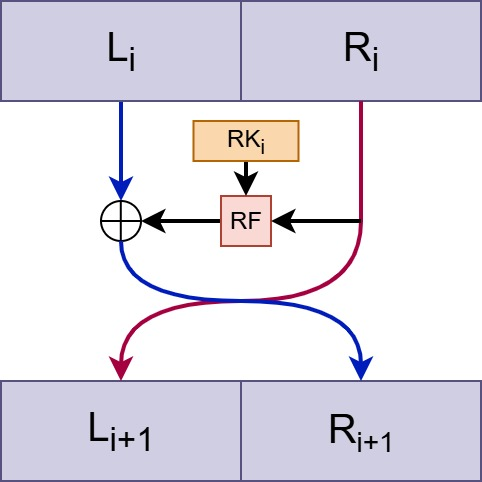
\includegraphics[width=0.5\linewidth]{img/feistel_round.jpg}
                    \caption{Feistel Network round}
                    \label{fig:placeholder}
                \end{figure}
                \item[Add-Rotate-XOR (ARX)\cite{sparx}] Classe di cifrari progettati utilizando soltanto semplici operazioni di \textit{addizione modulare} ($\boxplus$), \textit{rotazione} ($\lll, \ggg$) e \textit{XOR} ($\oplus$).
            \end{description}
            
            Di per sé, un cifrario a blocco non è una soluzione sicura, soprattutto in presenza di più blocchi da cifrare; presenta un comportamento deterministico: applica, a parità di chiave, sempre la stessa permutazione. Occorre adottare delle particolari tecniche, chiamate \textit{Modes of Operation}, che utilizzano il cifrario a blocco come primitiva e non come unica risorsa. \cite{handcypto, computernet}
            % modes
            
            \subsubsection{Cifrari a flusso}
            Un cifrario a flusso è un algoritmo che cifra un messaggio combinandolo con un flusso pseudocasuale di simboli (\textit{keystream}). Ogni simbolo del plaintext è cifrato con il simbolo corrispondente del keystream.\\
            La componente base di un cifrario a flusso è solitamente un \textit{LFSR} (\textit{linear-feedback shift register}), uno strumento utilizzato per la generazione pseudocasuale di numeri, con buone proprietà statistiche. Un LFSR consiste in un array di registri da un bit ciascuno, i cui valori ne rappresentano lo stato. Lo stato è aggiornato ad ogni intervallo dato, shiftando i valori dei registri verso destra, mentre il nuovo valore del primo registro da sinistra è calcolato tramite lo XOR di un sottoinsieme dei valori attuali. In un dato momento, il valore dell'ultimo registro a destra rappresenta l'output del LFSR.\cite{moderncrypto}
            \begin{figure}[htbp]
                \centering
                \begin{tikzpicture}[scale=1]
                	\node[rectangle,draw,minimum size=1cm] (r0) at (4,3) {$S_{\ell-1}$};
                	
                	\foreach \i in {1,...,6} {
                		\edef\p{\number\numexpr\i-1\relax}
                		\node[rectangle,draw,minimum size=1cm,right of =
                		r\p] (r\i) {};
                	};
                	
                	\node at (r1) {$S_{\ell-2}$};
                	\node at (r5) {$S_1$};
                	\node at (r6) {$S_0$};
                	
                	\node[XOR,thick,below=.75cm of r0] (x1) {};
                	\node[XOR,thick,below=.75cm of r1] (x2) {};
                	\node[XOR,thick,below=.75cm of r5] (x5) {};
                	
                	\draw[edge] (r5) -- (x5.north);
                	\draw[edge] (r1) -- (x2.north);
                	\draw[edge] (r0) -- (x1.north);
                	
                	\draw[edge] (r6) |- (x5.east);
                	\draw[edge,dotted] (x5.west) -- (x2.east);
                	\draw[edge] (x2) -- (x1);
                	\draw[edge] (x1.west) -- ++ (-1,0) |- (r0);
                	\draw[edge] (r6.east) -- ++ (1,0);
                \end{tikzpicture}
                \caption{LFSR}
                \label{fig:lfsr}
            \end{figure}
        \subsection{Crittografia Lightweight}
        I tradizionali metodi crittografici richiedono un utilizzo intensivo dello risorse computazionali. La necessità di soluzioni sicure per le infrastrutture IoT, caratterizzate ad un'ampia schiera di dispositivi con risorse limitate, ha reso necessaria la specializzazione di una branca della crittografia dedicata.
        
        La crittografia Lightweight (LWC, LightWeight Cryptography) si occupa di trovare soluzioni crittografiche leggere, con ridotto impatto su memoria, tempo di CPU e consumi energetici, in modo da poter offrire sicurezza anche ai dispositivi più limitati. La leggerezza è ottenuta solitamente sacrificando parte della sicurezza, tramite l'adozione di block size e chiavi ridotte oppure round meno complessi\cite{cryptometh}. La LWC riunisce un variegato insieme di soluzioni, in quanto, dato il numero elevato e la varietà dei dispositivi per cui è pensata, risulta difficile e controproducente ottenere una definizione univoca di cosa sia ``lightweight'', leggero. Infatti, un algoritmo crittografico potrà avere un'implementazione software, tramite un normale linguaggio di programmazione, oppure una hardware, in circuiti veri e propri (ASIC) o su FPGA; sulla base di questa distinzione emergono importanti differenze. Nel caso software, gli aspetti su cui rivolgere l'attenzione sono consumo di memoria e throughput; in hardware, invece, le metriche riguardano il circuito, e sono: latenza, consumo energetico e complessità Gate Equivalent (GE).

    \section{Sistemi embedded}
    Un sistema embedded può essere definito come ``un sistema informatico progettato e costruito esclusivamente per il suo scopo"\cite{embeddedsys}.
    I sistemi embedded spaziano tra i più disparati oggetti: dall'uso quotidiano (elettrodomestici), ai veicoli, ai sensori intelligenti (come nel caso di questa tesi), fino a scopi militari (missili).\\
    I computer \textit{integrati} in questi sistemi sono detti \textit{microcontrollori}\cite{architetture}.
    
    	\subsection{Vincoli}
    	Essendo progettati per un compito specifico, i sistemi embedded offrono meno supporto e presentano spesso numerosi vincoli. La necessità di produzione su larga scala e il fatto di rientrare nel budget del dispositivo in cui sono integrati richiedono ai progettisti un'attenta analisi dei \textit{costi}. La riduzione dei costi si riflette direttamente sui vincoli \textit{hardware} dei dispositivi, soprattutto in termini di RAM, ROM, velocità del processore, periferiche e consumo energetico. Come spesso accade, l'ottimizzazione di queste risorse risulta un problema complesso, richiedendo dei compromessi: codice più veloce richiede più spazio, aumentando la velocità della CPU aumentano di conseguenza i consumi, rimuovendo le periferiche non strettamente necessarie si guadagna in spazio e consumi, e molti altri.
    	Dal lato software, invece, possono essere richieste garanzie di \textit{real-time}, determinismo, oppure di tolleranza ai guasti.\cite{embeddedsys}
    	\subsection{Programmazione}
    	La sviluppo di codice embedded richiede diverse competenze, tra cui: conoscenza approfondita dell'hardware presente nel dispositivo, padronanza della programmazione a basso livello, soprattutto nella gestione della memoria, abilità nel bilanciare le richieste applicative con i vincoli del sistema.
    	Al contrario di quello che accade nei dispositivi general-purpose, inoltre, una errata gestione software può causare danni alle componenti hardware, anche gravi.
    		\subsubsection{Linguaggi}
    		Avendo risorse limitate, i sistemi embedded non sono dotati di compilatore, il codice che eseguono è \textit{cross-compilato} su un altro dispositivo e successivamente trasferito nella memoria integrata. I produttori di microprocessori solitamente forniscono ambienti di sviluppo dedicati con cross-compiler proprietari, ma sono presenti anche alternative GNU.
    		Le tool-chain embedded, nella maggior parte dei casi, supportano solo linguaggi come C o C++, con funzionalità e librerie limitate (es. supporto ridotto per aritmetica floating-point).
			\subsubsection{Debug}
			Altra questione delicata è quella del debugging, che, similmente alla compilazione, richiede un \textit{cross-debugger}. Questi particolari programmi sono eseguiti su un dispositivo esterno e comunicano con il microprocessore target tramite interfacce e periferiche dedicate (es. JTAG).
			Le funzionalità di debug devono essere esplicitamente supportate dal processore, attraverso hardware specifico, come per esempio registri riservati ai breakpoint (hardware breakpoint).
			
			\begin{figure}[h]
				\centering
				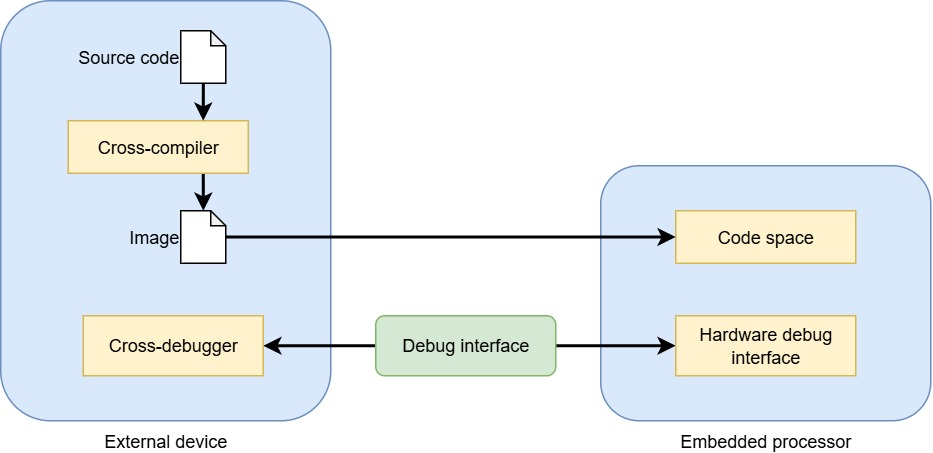
\includegraphics[width=0.5\linewidth]{img/cross-compiler-debugger.jpg}
				\caption{Comunicazione con microprocessore embedded}
				\label{fig:mcucomm}
			\end{figure}
			    		
\chapter{Algoritmi}
	\section{Cifrari a blocco}
		\subsection{AES}
		L'Advanced Encryption Standard specifica un algoritmo crittografico approvato dal FIPS (Federal Information Processing Standards), scelto al termine di una competizione indetta dal NIST (US National Institute of Standards and Technology), che vide come vincitore il cifrario presentato da Vincent Rijmen e Joan Daemen: Rijndael\cite{aes}. Sia durante il processo di selezione che dopo essere stato adottato come standard, questo algoritmo ha ricevuto un intenso studio da parte dei crittoanalisti. Anche per questo motivo, AES risulta una scelta eccellente per sistemi che richiedano segretezza: libero, standardizzato, efficiente e altamente sicuro. \cite{moderncrypto}
			\subsubsection{Design}
			Le operazioni dell'algoritmo sono effettuate su un array bi-dimensionale ($4 \times 4$), definito state. Ogni byte $s_{r,c}$ dello state ha due indici: di riga $r$ e di colonna $c$. Il cuore dell'algoritmo è caratterizzato da una serie di round, durante cui, in sequenza, vengono applicate queste trasformazioni:
			\begin{itemize}
				\item \Call{SubBytes}{\null} : trasformazione invertibile e non-lineare, descritta da una S-box e ottenuta tramite la sostituzione indipendente dei byte dello state:
				\[s'_{r,c} = \Call{SBox}{s_{r,c}}\]
				\begin{table}[h!]
					\centering
					\caption{SBox():}
					\begin{tabular}{|c|cccccccccccccccc|}
						\hline
						& .0 & .1 & .2 & .3 & .4 & .5 & .6 & .7 & .8 & .9 & .a & .b & .c & .d & .e & .f \\
						\hline
						0. & 63 & 7c & 77 & 7b & f2 & 6b & 6f & c5 & 30 & 01 & 67 & 2b & fe & d7 & ab & 76 \\
						1. & ca & 82 & c9 & 7d & fa & 59 & 47 & f0 & ad & d4 & a2 & af & 9c & a4 & 72 & c0 \\
						2. & b7 & fd & 93 & 26 & 36 & 3f & f7 & cc & 34 & a5 & e5 & f1 & 71 & d8 & 31 & 15 \\
						3. & 04 & c7 & 23 & c3 & 18 & 96 & 05 & 9a & 07 & 12 & 80 & e2 & eb & 27 & b2 & 75 \\
						4. & 09 & 83 & 2c & 1a & 1b & 6e & 5a & a0 & 52 & 3b & d6 & b3 & 29 & e3 & 2f & 84 \\
						5. & 53 & d1 & 00 & ed & 20 & fc & b1 & 5b & 6a & cb & be & 39 & 4a & 4c & 58 & cf \\
						6. & d0 & ef & aa & fb & 43 & 4d & 33 & 85 & 45 & f9 & 02 & 7f & 50 & 3c & 9f & a8 \\
						7. & 51 & a3 & 40 & 8f & 92 & 9d & 38 & f5 & bc & b6 & da & 21 & 10 & ff & f3 & d2 \\
						8. & cd & 0c & 13 & ec & 5f & 97 & 44 & 17 & c4 & a7 & 7e & 3d & 64 & 5d & 19 & 73 \\
						9. & 60 & 81 & 4f & dc & 22 & 2a & 90 & 88 & 46 & ee & b8 & 14 & de & 5e & 0b & db \\
						a. & e0 & 32 & 3a & 0a & 49 & 06 & 24 & 5c & c2 & d3 & ac & 62 & 91 & 95 & e4 & 79 \\
						b. & e7 & c8 & 37 & 6d & 8d & d5 & 4e & a9 & 6c & 56 & f4 & ea & 65 & 7a & ae & 08 \\
						c. & ba & 78 & 25 & 2e & 1c & a6 & b4 & c6 & e8 & dd & 74 & 1f & 4b & bd & 8b & 8a \\
						d. & 70 & 3e & b5 & 66 & 48 & 03 & f6 & 0e & 61 & 35 & 57 & b9 & 86 & c1 & 1d & 9e \\
						e. & e1 & f8 & 98 & 11 & 69 & d9 & 8e & 94 & 9b & 1e & 87 & e9 & ce & 55 & 28 & df \\
						f. & 8c & a1 & 89 & 0d & bf & e6 & 42 & 68 & 41 & 99 & 2d & 0f & b0 & 54 & bb & 16 \\
						\hline
					\end{tabular}
				\end{table}
				\item \Call{ShiftRows}{\null} : shift dei byte che compongono le ultime tre righe dello state, il numero di posizioni dipende dall'indice della riga:
				\[s'_{r,c} = s_{r,(c+r) \bmod 4}\]
				\item \Call{MixColumns}{\null} : moltiplicazione, in $GF(2^8)$ definito da $x^8+x^4+x^3+x+1$, tra lo state e la matrice fissata:
				\[
				\begin{pmatrix}
					02 & 03 & 01 & 01 \\
					01 & 02 & 03 & 01 \\
					01 & 01 & 02 & 03 \\
					03 & 01 & 01 & 02 \\
				\end{pmatrix}
				\]
				\item \Call{AddRoundKey}{\null} : somma (bitwise XOR) tra ciascuna colonna e la relativa word della round key corrispondente:
				\[[s'_{0,c},s'_{1,c},s'_{2,c},s'_{3,c}] = [s_{0,c},s_{1,c},s_{2,c},s_{3,c}] \oplus w_{(4*round+c)}\]
			\end{itemize}
			
			\begin{algorithm}
				\caption{Pseudocodice AES}
				\begin{algorithmic}
					\Procedure{Cipher}{$in, Nr, w$}
						\State {$state \gets in$}
						\State {$state \gets \Call{AddRoundKey}{state,w[0 \cdots 3]}$}
						\For{$round=1$ \textbf{to} $Nr-1$}
							\State {$state \gets \Call{SubBytes}{state}$}
							\State {$state \gets \Call{ShiftRows}{state}$}
							\State {$state \gets \Call{MixColumns}{state}$}
							\State {$state \gets \Call{AddRoundKey}{state,w[4*round \cdots 4*round+3]}$}
						\EndFor
						\State {$state \gets \Call{SubBytes}{state}$}
						\State {$state \gets \Call{ShiftRows}{state}$}
						\State {$state \gets \Call{AddRoundKey}{state,w[4*Nr \cdots 4*Nr+3]}$}
						\State {\textbf{return} $state$}
					\EndProcedure
				\end{algorithmic}
			\end{algorithm}
			
			Le round key sono generate tramite la procedura \Call{KeyExpansion}{\null}, in modo ricorsivo, a partire dalla chiave principale.\\
			In questa fase, due sono le trasformazioni applicate:
			\begin{align*}
			&\Call{RotWord}{[a_0,a_1,a_2,a_3]} = [a_1,a_2,a_3,a_0],\\
			&\Call{SubWord}{[a_0,a_1,a_2,a_3]} = [S(a_0),S(a_1), S(a_2), S(a_3)].
			\end{align*}

			\begin{algorithm}
				\caption{Pseudocodice Key Expansion}
				\begin{algorithmic}
					\Procedure{KeyExpansion}{key}
						\State {$i \gets 0$}
						\While{$i \le Nk-1 $}
							\State {$w[i] \gets key[i]$}
							\State {$i \gets i+1$}
						\EndWhile
						\While{$i \le 4*Nr + 3$}
							\State {$temp \gets w[i-1]$}
							\If{$i \bmod Nk = 0$}
								\State {$temp \gets \Call{SubWord}{}(\Call{RotWord}{temp}) \oplus Rcon[i/Nk]$}
							\ElsIf{$(Nk \gtr 6) \wedge (i \bmod Nk = 4)$}
								\State {$temp \gets \Call{SubWord}{temp}$}
							\EndIf
							\State {$w[i] \gets w[i - Nk] \oplus temp$}
							\State {$i \gets i+1$}
						\EndWhile
						\State {\textbf{return} $w$}
					\EndProcedure
				\end{algorithmic}
			\end{algorithm}

			\subsubsection{Crittoanalisi}
			\begin{center}
				\begin{tabular}{ |c|c|c|c|c|c| } 
					\hline
					Attacco & Rounds & Dati & Memoria & Tempo & Fonte \\ 
					\hline
					\hline
					Biclique (AES-128) & 10 & $2^{88}$ & $2^8$ & $2^{126.18}$ & \cite{aes_biclique} \\ 
					\hline
					Related-key (AES-256) & 14 & $2^{99.5}$ & $2^{77}$ & $2^{99.5}$ & \cite{aes_relatedkey}\\ 
					\hline
					Side channel & & & & & \cite{aesside, aesfault}\\
					\hline
				\end{tabular}
			\end{center}
		\subsection{CLEFIA}
		CLEFIA è un cifrario proprietario sviluppato da Sony, sfruttando le ultime scoperte in ambito di crittanalisi \cite{clefia}.
			\subsubsection{Design}
			La struttura base è data da una particolare estensione di rete Feistel (Type-2 generalized Fesitel network): a 4-rami e con due funzioni ($F_0, F_1$) per round. Queste funzioni adottano \textit{Diffusion Switching Mechanism}\cite{clefiadsm}: utilizzano due diverse matrici di diffusione per aumentare l'immunità ad attacchi differenziali e lineari.
			
			La struttura della particolare rete Feistel adottata è descritta come:\\
			\begin{algorithm}[htbp]
				\caption{Generaized Fesitel Network}
				\begin{algorithmic}
					\Procedure{$GFN_{4,r}$}{$RK, X$}
						\State {$T \gets X$}
						\For{$i=0$ \textbf{to} $r-1$}
							\State {$T_1 \gets T_1 \oplus F_0(RK_{2i},T_0)$}
							\State {$T_3 \gets T_3 \oplus F_1(RK_{2i+1},T_2)$}
							\State {$T \gets T_1||T_2||T_3||T_0$}
						\EndFor
						\State {\textbf{return} $T_3||T_0||T_1||T_2$}
					\EndProcedure
				\end{algorithmic}
			\end{algorithm}
			
			\begin{minipage}[c]{0.45\textwidth}
				\noindent
				\centering
				\begin{algorithm}[H]
					\caption{$F_0$}
					\begin{algorithmic}
						\Procedure{$F_0$}{$RK,x$}
						\State {$T \gets RK \oplus x$}
						\State {$T \gets S_0(T_0)||S_1(T_1)||S_0(T_2)||S_1(T_3)$}
						\State {\textbf{return} $M_0 \times ^tT$}
						\EndProcedure
					\end{algorithmic}
				\end{algorithm}
			\end{minipage}
			\begin{minipage}[c]{0.45\textwidth}
				\noindent
				\centering
				\begin{algorithm}[H]
					\caption{$F_1$}
					\begin{algorithmic}
						\Procedure{$F_1$}{$RK,x$}
						\State {$T \gets RK \oplus x$}
						\State {$T \gets S_1(T_0)||S_0(T_1)||S_1(T_2)||S_0(T_3)$}
						\State {\textbf{return} $M_1 \times ^tT$}
						\EndProcedure
					\end{algorithmic}
				\end{algorithm}
			\end{minipage}\\
			Le due matrici sono:
			\[M_0 =
				\begin{pmatrix}
					01 & 02 & 04 & 06\\
					02 & 01 & 06 & 04\\
					04 & 06 & 01 & 02\\
					06 & 04 & 02 & 01
				\end{pmatrix},
			M_1 = 
				\begin{pmatrix}
					01 & 08 & 02 & 0a\\
					08 & 01 & 0a & 02\\
					02 & 0a & 01 & 08\\
					0a & 02 & 08 & 01
				\end{pmatrix}
			\]
			Le moltiplicazioni sono eseguite in $GF(2^8)$ definito da $z^8+z^4+z^3+z^2+1$
			
			Sono inoltre presenti due S-box, basate su strutture algebriche differenti, scelta che \textit{prevede} di aumentare la resistenza ad attacchi algebrici.
			\begin{table}[h!]
				\centering
				\caption{S-boxes $S_0$ e $S_1$}
				\scriptsize
				\setlength{\tabcolsep}{2pt} % regola la spaziatura tra le colonne
				\begin{tabular*}{\textwidth}{@{\extracolsep{\fill}}|c|llllllllllllllll|llllllllllllllll|}
					\hline
					& \multicolumn{16}{c|}{$S_0$} & \multicolumn{16}{c|}{$S_1$} \\
					& .0 & .1 & .2 & .3 & .4 & .5 & .6 & .7 & .8 & .9 & .a & .b & .c & .d & .e & .f &
					.0 & .1 & .2 & .3 & .4 & .5 & .6 & .7 & .8 & .9 & .a & .b & .c & .d & .e & .f \\
					\hline
					0. & 57 & 49 & d1 & c6 & 2f & 33 & 74 & fb & 95 & 6d & 82 & ea & 0e & b0 & a8 & 1c & 6c & da & c3 & e9 & 4e & 9d & 0a & 3d & b8 & 36 & b4 & 38 & 13 & 34 & 0c & d9 \\
					1. & 28 & d0 & 4b & 92 & 5c & ee & 85 & b1 & c4 & 0a & 76 & d6 & 3f & 91 & 7a & 0f & bf & 74 & 94 & 8f & b7 & 9c & e5 & dc & 9e & 07 & 49 & 4f & 98 & 2c & b0 & 93 \\
					2. & bf & a1 & 19 & 65 & f7 & 7a & 32 & 20 & 06 & ce & e4 & 83 & 9d & 5b & 4c & d8 & 12 & eb & cd & b3 & 92 & e7 & 41 & 60 & e3 & 21 & 27 & 3b & e6 & 19 & d2 & 0e \\
					3. & 42 & 5d & 2e & e8 & d4 & 9b & 0f & 13 & 3c & 89 & 67 & c0 & 71 & aa & b6 & f5 & 91 & 11 & c7 & 3f & 2a & 8e & a1 & bc & 2b & c8 & c5 & 0f & 5b & f3 & 87 & 8b \\
					4. & a4 & be & fd & 8c & 12 & 00 & 97 & da & 78 & e1 & cf & 6b & 39 & 43 & 55 & 26 & fb & f5 & de & 20 & c6 & a7 & 84 & ce & d8 & 65 & 51 & c9 & a4 & ef & 43 & 53 \\
					5. & 30 & 98 & cc & dd & eb & 54 & b3 & 8f & 4e & 16 & fa & 22 & a5 & 77 & 09 & 61 & 25 & 5d & 9b & 31 & e8 & 3e & 0d & d7 & 80 & ff & 69 & 8a & ba & 0b & 73 & 5c \\
					6. & d6 & 2a & 53 & 37 & 45 & c1 & 6c & ae & ef & 70 & 08 & 99 & 8b & 1d & f2 & b4 & 6e & 54 & 15 & 62 & f6 & 35 & 30 & 52 & a3 & 16 & d3 & 28 & 32 & fa & aa & 5e \\
					7. & e9 & c7 & 9f & 4a & 31 & 25 & fe & 7c & d3 & a2 & bd & 56 & 14 & 88 & 60 & 0b & cf & ea & ed & 78 & 33 & 58 & 09 & 7b & 63 & c0 & c1 & 46 & 1e & df & a9 & 99 \\
					8. & cd & e2 & 34 & 50 & 9e & dc & 11 & 05 & 2b & b7 & a9 & 48 & ff & 66 & 8a & 73 & 55 & 04 & c4 & 86 & 39 & 77 & 82 & ec & 40 & 18 & 90 & 97 & 59 & dd & 83 & 1f \\
					9. & 03 & 75 & 86 & f1 & 6a & a7 & 40 & c2 & b9 & 2c & db & 1f & 58 & 94 & 3e & ed & 9a & 37 & 06 & 24 & 64 & 7c & a5 & 56 & 48 & 08 & 85 & d0 & 61 & 26 & ca & 6f \\
					a. & fc & 1b & a0 & 04 & b8 & 8d & e6 & 59 & 62 & 93 & 35 & 7e & ca & 21 & df & 47 & 7e & 6a & b6 & 71 & a0 & 70 & 05 & d1 & 45 & 8c & 23 & 1c & f0 & ee & 89 & ad \\
					b. & 15 & f3 & ba & 7f & a6 & 69 & c8 & 4d & 87 & 3b & 9c & 01 & e0 & de & 24 & 52 & 7a & 4b & c2 & 2f & db & 5a & 4d & 76 & 67 & 17 & 2d & f4 & cb & b1 & 4a & a8 \\
					c. & 7b & 0c & 68 & 1e & 80 & b2 & 5a & e7 & ad & d5 & 23 & f4 & 46 & 3f & 91 & c9 & b5 & 22 & 47 & 3a & d5 & 10 & 4c & 72 & cc & 00 & f9 & e0 & fd & e2 & fe & ae \\
					d. & 6e & 84 & 72 & bb & 0d & 18 & d9 & 96 & f0 & 5f & 41 & ac & 27 & c5 & e3 & 3a & f8 & 5f & ab & f1 & 1b & 42 & 81 & d6 & be & 44 & 29 & a6 & 57 & b9 & af & f2 \\
					e. & 81 & 6f & 07 & a3 & 79 & f6 & 2d & 38 & 1a & 44 & 5e & b5 & d2 & ec & cb & 90 & d4 & 75 & 66 & bb & 68 & 9f & 50 & 02 & 01 & 3c & 7f & 8d & 1a & 88 & bd & ac \\
					f. & 9a & 36 & e5 & 29 & c3 & 4f & ab & 64 & 51 & f8 & 10 & d7 & bc & 02 & 7d & 8e & f7 & e4 & 79 & 96 & a2 & fc & 6d & b2 & 6b & 03 & e1 & 2e & 7d & 14 & 95 & 1d \\
					\hline
				\end{tabular*}
			\end{table}
				
			\begin{algorithm}
				\caption{pseudocodice CLEFIA}
				\begin{algorithmic}
					\Procedure{Clefia$_r$}{$WK,RK,P$}
					\State {$T \gets P_0||(P_1 \oplus WK_0)||P_2||(P_3 \oplus WK_1)$}
					\State {$T \gets GFN_{4,r}(RK,T)$}
					\State {\textbf{return} $T_0||(T_1 \oplus WK_2)||T_2||(T_3 \oplus WK_3)$}
					\EndProcedure
				\end{algorithmic}
			\end{algorithm}

			La key schedule è divisa in due fasi:
			\begin{enumerate}
				\item generazione di una chiave intermedia \textit{L}
				\item espansione di \textit{L} per generare whitening key $WK$ e round key $RK_i$
			\end{enumerate}
			
			Sono necessarie 60 costanti $CON_i$, generate nel seguente modo:
			\begin{algorithm}
				\caption{Generazione $CON_i$}
				\begin{algorithmic}
					\State {$T \gets \mathtt{0x428a}$}
					\For{$i=0$ \textbf{to} $29$}
						\State {$CON_{2i} \gets (T \oplus \mathtt{0xb7e1}) | (\overline{T} \lll 1)$}
						\State {$CON_{2i+1} \gets (\overline{T} \oplus \mathtt{0x243f}) | (T \lll 8)$}
						\State {$T \gets T \cdot 0x0002^{-1}$}
					\EndFor
				\end{algorithmic}
			\end{algorithm}\\
			La moltiplicazione nell'ultimo step è fatta in $GF(2^{16})$ definito da $z^{16}+z^{15}+z^{13}+z^{11}+z^5+z^4+1$.
			\begin{algorithm}
				\caption{pseudocodice Key Expansion CLEFIA-128}
				\begin{algorithmic}
					\Procedure{KeyExpansion}{K}
						\State {$L \gets GFN_{4,12}(CON_{0..23}, K)$}
						\State {$WK \gets K$}
						\For{$i = 0$ \textbf{to} $8$}
							\State {$T \gets L \oplus (CON_{24+4i}||CON_{24+4i+1}||CON_{24+4i+2}||CON_{24+4i+3})$}
							\State {$L \gets L[7..63] || L[121..127] || L[0..6] || L[64..120]$}
							\If{$i$ is odd}
								\State {$T \gets T \oplus K$}
							\EndIf
							\State {$RK_{4i} \gets T$}
						\EndFor
					\EndProcedure
				\end{algorithmic}
			\end{algorithm}
			
			\subsubsection{Crittoanalisi}
			Diversi studi consentono di affermare che Clefia è resistente alle moderne tecniche di crittoanalisi.\cite{clefiaanal}
			\begin{center}
				\begin{tabular}{ |c|c|c|c|c|c| } 
					\hline
					Attacco & Rounds & Dati & Memoria & Tempo & Fonte \\ 
					\hline 
					\hline
					Impossible differential & 12 & $2^{118.9}$ & $2^{73}$ & $2^{119}$ & \cite{clefiadiff} \\
					\hline
					Side channel & & & & & \cite{clefiafault}\\
					\hline
				\end{tabular}
			\end{center}
		\subsection{LEA}
		Lightweight Encryption Algorithm (LEA) è un cifrario sviluppato dalla Corea del Sud, da cui è inoltre adottato come standard nazionale. Obiettivo principale è quello di risultare efficiente sia in implementazioni software che in quelle hardware\cite{lea}.
			\subsubsection{Design}
			LEA consiste di sole operazioni ARX su word di 32 bit. La word-size è stata scelta dai progettisti sulla base della convinzione che in futuro le operazioni a 32 bit saranno implementate efficientemente anche su dispositivi con risorse limitate.
			La cifratura è divisa in tre fasi: inizializzazione, round iterativi e finalizzazione.
			\begin{algorithm}
				\caption{pseudocodice LEA}
				\begin{algorithmic}
					\Procedure{LEA}{P,RK}
						\State {$X_0 \gets P$}
						\For{$i=0$ \textbf{to} $r-1$}
							\State {$X_{i+1}[0] \gets LROT_9((X_i[0] \oplus RK_i[0]) \boxplus (X_i[1] \oplus RK_i[1]))$}
							\State {$X_{i+1}[1] \gets RROT_5((X_i[1] \oplus RK_i[2]) \boxplus (X_i[2] \oplus RK_i[3]))$}
							\State {$X_{i+1}[2] \gets RROT_3((X_i[2] \oplus RK_i[4]) \boxplus (X_i[3] \oplus RK_i[5]))$}
							\State {$X_{i+1}[3] \gets X_i[0]$}
						\EndFor
						\State {$C \gets X_r$}
						\State {\textbf{return} $C$}
					\EndProcedure
				\end{algorithmic}
			\end{algorithm}
			
			La struttura della key schedule è semplice, senza mix tra word diverse o avalanche effect, ma non per questo poco sicura. Come per la cifratura, le operazioni sono ARX, con l'aggiunta dell'utilizzo di costanti $\delta$:
			\begin{align*}
				\delta[0] = \mathtt{0xc3efe9db},\quad \delta[1] = \mathtt{0x44626b02},\\
				\delta[2] = \mathtt{0x79e27c8a},\quad \delta[3] = \mathtt{0x78df30ec},\\
				\delta[4] = \mathtt{0x715ea49e},\quad \delta[5] = \mathtt{0xc785da0a},\\
				\delta[6] = \mathtt{0xe04ef22a},\quad \delta[7] = \mathtt{0xe5c40957}.
			\end{align*}
			La semplicità è ancora una volta ricercata per consentire implementazioni efficienti.
			\begin{algorithm}
				\caption{pseudocodice key schedule LEA-128}
				\begin{algorithmic}
					\Procedure{KeySchedule}{K}
						\State {$T \gets K$}
						\For{$i = 0$ \textbf{to} 23}
							\State {$T[0] \gets LROT_1(T[0] \boxplus LROT_i(\delta[i \bmod 4]))$}
							\State {$T[1] \gets LROT_3(T[1] \boxplus LROT_{i+1}(\delta[i \bmod 4]))$}
							\State {$T[2] \gets LROT_6(T[2] \boxplus LROT_{i+2}(\delta[i \bmod 4]))$}
							\State {$T[3] \gets LROT_{11}(T[3] \boxplus LROT_{i+3}(\delta[i \bmod 4]))$}
							\State {$RK_i \gets T[0]||T[1]||T[2]||T[1]||T[3]||T[1]$}
						\EndFor
					\EndProcedure
				\end{algorithmic}
			\end{algorithm}
			
			\subsubsection{Crittoanalisi}
			Lo sviluppo di LEA è stato guidato anche dall'obiettivo di resistere a tutti gli attacchi esistenti e garantire un certo margine di sicurezza futura. Sia $R$ il numero minimo di round per resistere a tutte le tecniche di crittoanalisi, LEA ne prevede $3R/2$ in previsione di nuove tipologie di attacchi che potrebbero emergere in futuro.\\
			Al momento non esistono attacchi full-round noti.
			\begin{center}
				\begin{tabular}{ |c|c|c|c|c|c| } 
					\hline
					Attacco & Rounds & Dati & Memoria & Tempo & Fonte \\ 
					\hline 
					\hline
					Differential & 13 & $2^{127}$ & $2^{22}$ & $2^{127}$ & \cite{leadiff} \\
					\hline
					Boomerang & 15 & $2^{116.3}$ & & & \cite{lea} \\
					\hline
				\end{tabular}
			\end{center}
		\subsection{PRINCE}
		\label{ssec:prince}
			PRINCE è un cifrario ottimizzato rispetto alla latenza su  hardware; consente infatti implementazioni full-unrolled, con cifratura in un solo ciclo di clock\cite{prince}.
			\subsubsection{Design}
			L'obiettivo dei progettisti di PRINCE era creare un cifrario sulla base dei seguenti criteri: cifratura istantanea, bassa latenza, costi hardware moderati, decifratura ottenibile con minor overhead possibile.
			Per ottenere i primi due, sono necessari round in numero ridotto e con logica non troppo complessa: un critical-path leggero consente infatti di impiegare una velocità di clock maggiore.
			Gli ultimi due criteri, invece, sono consentite grazie alla particolare proprietà di $\alpha$-reflection: la decifratura corrisponde ad un cifratura con una chiave ricavata da quella principale.\\
			PRINCE è un cifrario a blocchi di 64 bit, con una chiave da 128 bit $k = k_0 || k_1$. La chiave è estesa a 192 bit:
			\[(k_0||k'_0||k_1) := (k_0 || (k_0 \ggg 1) \oplus (k_0 \gg 63) || k_1)\]\\
			La struttura base è detta \textit{FX-construction}: le sotto chiavi $k_0$ e $k'_0$ sono usate come whitening key, mentre $k_1$ è usata nei 12 round del costrutto chiamato PRINCE$_{core}$.
			\begin{figure}[h!]
				\centering
				\begin{tikzpicture}[scale=1]
					
					\tikzstyle{every node}=[transform shape];
					\tikzstyle{every node}=[node distance=2.0cm];
					
					% data path
					\node (XOR-1)[XOR,scale=1] {};
					\node [left of=XOR-1] (p) {$m$};
					\node (f-1) [right of=XOR-1,draw,rectangle,thick,minimum width=1.5em] {PRINCE$_{core}$};
					\path[line] (p) edge (XOR-1);
					\path[line] (XOR-1) edge (f-1);  
					
					\node (XOR-2)[right of=f-1,XOR,scale=1] {};
					\path[line] (f-1) edge (XOR-2);
					\node (f-2) [right of=XOR-2] {};
					\path[line] (XOR-2) edge (f-2) ;
					\node [right of=XOR-2,node distance=2.1cm] {$c$};
					
					%% Subkeys
					\node (k-0) [above=0.6cm of XOR-1] {};
					\path[line] (k-0) node[above] {\small $k_{0}$} edge (XOR-1);
					
					\node (k-1) [above=0.6cm of XOR-2] {};
					\path[line] (k-1) node[above] {\small $k'_{0}$} edge (XOR-2);
					
				\end{tikzpicture}
				\caption{PRINCE FX-construct}
				\label{fig:princefx}
			\end{figure}
			
			Ogni round prevede le seguenti trasformazioni dello stato:
			\begin{enumerate}
				\item \textbf{$k_1$-add}: somma (XOR) con la sotto-chiave.
				\item \textbf{S-Layer}: sostituzione con S-box $S$ a 4 bit:
				\begin{center}
					\begin{tabular}{|c|cccccccccccccccc|}
						\hline
						$x$ & $\mathtt{0}$ & $\mathtt{1}$ & $\mathtt{2}$ & $\mathtt{3}$ & $\mathtt{4}$ & $\mathtt{5}$ & $\mathtt{6}$ & $\mathtt{7}$ & $\mathtt{8}$ & $\mathtt{9}$ & $\mathtt{a}$ & $\mathtt{b}$ & $\mathtt{c}$ & $\mathtt{d}$ & $\mathtt{e}$ & $\mathtt{f}$\\
						$S(x)$ & $\mathtt{b}$ & $\mathtt{f}$ & $\mathtt{3}$ & $\mathtt{2}$ & $\mathtt{a}$ & $\mathtt{c}$ & $\mathtt{9}$ & $\mathtt{1}$ & $\mathtt{6}$ & $\mathtt{7}$ & $\mathtt{8}$ & $\mathtt{0}$ & $\mathtt{e}$ & $\mathtt{5}$ & $\mathtt{d}$ & $\mathtt{4}$\\
						\hline
					\end{tabular}
				\end{center}
				\item \textbf{(M/M')-Layer}: moltiplicazione con matrice $M$ o $M'$. Essendo usata nel round centrale, $M'$ deve essere un'involuzione; $M$ si ottiene invece con la combinazione tra $M'$ e una permutazione $SR$: $M = SR \circ M' $.
				\[SR:(0,1,2,3,4,5,6,7,8,9,10,11,12,13,14,15) \rightarrow (0,5,10,15,4,9,14,3,8,13,2,7,12,1,6,11) \]
				Le seguenti matrici sono utilizzate per costruire $M'$:
				\[M_0 = 
				\begin{pmatrix}
					0000\\
					0100\\
					0010\\
					0001
				\end{pmatrix},
				M_1 =
				\begin{pmatrix}
					1000\\
					0000\\
					0010\\
					0001
				\end{pmatrix},
				M_2 =
				\begin{pmatrix}
					1000\\
					0100\\
					0000\\
					0001
				\end{pmatrix},
				M_3 =
				\begin{pmatrix}
					1000\\
					0100\\
					0010\\
					0000
				\end{pmatrix}
				\]
				Da cui:
				\[ \hat{M^{(0)}} = 
				\begin{pmatrix}
					M_0\ M_1\ M_2\ M_3\\
					M_1\ M_2\ M_3\ M_0\\
					M_2\ M_3\ M_0\ M_1\\
					M_3\ M_0\ M_1\ M_2
				\end{pmatrix},
				\hat{M^{(1)}} = 
				\begin{pmatrix}
					M_1\ M_2\ M_3\ M_0\\
					M_2\ M_3\ M_0\ M_1\\
					M_3\ M_0\ M_1\ M_2\\
					M_0\ M_1\ M_2\ M_3
				\end{pmatrix}
				\]
				Infine, $M'$ è ottenuta costruendo una matrice $64 \times 64$ con $(\hat{M^{(0)}} , \hat{M^{(1)}}, \hat{M^{(1)}}, \hat{M^{(0)}})$ come blocchi diagonali.
				\item \textbf{$RC_i$-add}: somma (XOR) con la relativa costante. Le costanti sono scelte in modo che per $0 \le i \le 11$, $RC_i \oplus RC_{11-i} = \alpha = \mathtt{0xc0ac29b7c97c50dd}$; $RC_0 = 0$ e $RC_{1...5}$ sono derivate dalla parte decimale di $\pi$.
				\begin{center}
					\begin{tabular}{|c||c|}
						\hline
						$RC_0$ & $\mathtt{0000000000000000}$ \\
						$RC_1$ & $\mathtt{13198a2e03707344}$ \\
						$RC_2$ & $\mathtt{a4093822299f31d0}$ \\
						$RC_3$ & $\mathtt{082efa98ec4e6c89}$ \\
						$RC_4$ & $\mathtt{452821e638d01377}$ \\
						$RC_5$ & $\mathtt{be5466cf34e90c6c}$ \\
						$RC_6$ & $\mathtt{7ef84f78fd955cb1}$ \\
						$RC_7$ & $\mathtt{85840851f1ac43aa}$ \\
						$RC_8$ & $\mathtt{c882d32f25323c54}$ \\
						$RC_9$ & $\mathtt{64a51195e0e3610d}$ \\
						$RC_{10}$ & $\mathtt{d3b5a399ca0c2399}$ \\
						$RC_{11}$ & $\mathtt{c0ac29b7c97c50dd}$ \\
						\hline
					\end{tabular}
				\end{center}
			\end{enumerate}
				\begin{figure}[h!]
				\centering
				\begin{tikzpicture}[scale=0.20]
					
					\draw[->,thick] (-7,2) -- ++(2,0);
					\draw[->,thick] (-5,2) -- ++(5,0);
					
					\foreach \x in {0,...,5} {
						\def \z{5*\x}
						\draw[thick] (\z,0) rectangle node[]{$\mathcal{R}_{\x}$} ++(3.5,4);
						\draw[->,thick] (\z+3.5,2) -- ++(1.5,0);
						\draw[->] (\z+1.75,5.5) -- ++(0,-1.5);
						\draw[] (\z+1.75,6.25) node[]{\scriptsize $RC_{\x}$} ++(0,0);
					}
					
					\def \z{5*6}
					\draw[thick] (\z,0.5) rectangle node[]{\tiny $SR^{\textnormal{\tiny -1}}$} ++(3,3);
					\draw[->,thick] (\z+3,2) -- ++(1,0);
					\def \z{5*6+4}
					\draw[thick] (\z,0.5) rectangle node[]{\tiny $M'$} ++(3,3);
					\draw[->,thick] (\z+3,2) -- ++(1,0);
					\def \z{5*6+8}
					\draw[thick] (\z,0.5) rectangle node[]{\tiny $SR$} ++(3,3);
					
					\foreach \x in {6,...,11} {
						\def \z{5*6+12.5+5*\x - 5*6}
						\draw[->,thick] (\z+3.5-5,2) -- ++(1.5,0);
						\draw[thick] (\z,0) rectangle node[]{$\mathcal{R}^{\textnormal{\tiny -1}}_{\x}$} ++(3.5,4);
						\draw[->] (\z+1.75,5.5) -- ++(0,-1.5);
						\draw[] (\z+1.75,6.25) node[]{\scriptsize $RC_{\x}$} ++(0,0);
					}
					
					\def \z{5*6+12.5+5*12 - 5*6}
					\draw[->,thick] (\z+3.5-5,2) -- ++(3,0);
					\draw[->,thick] (\z+6.5-5,2) -- ++(4,0);
					
					\draw[style=dashed] (-2,-9) rectangle ++(5*6+12.5+5*12 - 5*6 +2.5 ,17);
					\draw[] (5*6+4+1.5 ,8.5) node[above]{$\texttt{PRINCE}_{core}$} ++(0,0);
					
					\draw[thick] (-4,2) circle (1);
					\draw[thick] (-4,3) -- ++(0,-2);
					\draw[->,thick] (-4,6) -- ++(0,-3);
					\draw[] (-4,6) node[above]{$k_0$} ++(0,0);
					\draw[thick] (5*6+12.5+5*12 - 5*6 +2.5,2) circle (1);
					\draw[thick] (5*6+12.5+5*12 - 5*6 +2.5,3) -- ++(0,-2);
					\draw[->,thick] (5*6+12.5+5*12 - 5*6 +2.5,6) -- ++(0,-3);
					\draw[] (5*6+12.5+5*12 - 5*6 +2.5,6) node[above]{$k'_0$} ++(0,0);
					
					\def \z{5*3}
					\draw[->] (\z-4,-6) -- ++(3.5,0);
					\draw[] (\z,-6) circle (0.5);
					\draw[-] (\z,-5.5) -- ++(0,-1);
					\draw[->] (\z-0.5,-6) -- ++(2,0);
					\draw[] (\z+2.0,-6) circle (0.5);
					\draw[-] (\z+2.0,-5.5) -- ++(0,-1);
					\draw[->] (\z+1.5,-6) -- ++(2.0,0);
					
					\draw[->] (\z,-4) -- ++(0,-1.5);
					\draw[] (\z,-4.25) node[above]{\tiny $k_1$} ++(0,0);
					\draw[->] (\z+2.0,-4) -- ++(0,-1.5);
					\draw[] (\z+2.0,-4.25) node[above]{\tiny $RC_i$} ++(0,0);
					
					\draw[] (\z+3.5,-6-1.5) rectangle node[]{\tiny $S$} ++(3,3);
					\draw[->] (\z+6.5,-6) -- ++(1,0);
					\draw[] (\z+7.5,-6-1.5) rectangle node[]{\tiny $M$} ++(3,3);
					\draw[->] (\z+10.5,-6) -- ++(4,0);
					
					\draw[-,style=dashed] (\z-4+0.5,-5.5) -- (\z-0.5,-0.5);
					\draw[-,style=dashed] (\z+14.5-0.5,-5.5) -- (\z+3.5+0.5,-0.5);s
					
					\def \z{5*6+12.5+5*8 - 5*6}
					\draw[->] (\z+3,-6) -- ++(4.5,0);
					\draw[] (\z+3.5,-6) circle (0.5);
					\draw[-] (\z+3.5,-5.5) -- ++(0,-1);
					\draw[->] (\z+1,-6) -- ++(2,0);
					\draw[] (\z+1.5,-6) circle (0.5);
					\draw[-] (\z+1.5,-5.5) -- ++(0,-1);
					\draw[->] (\z,-6) -- ++(1.0,0);
					
					\draw[->] (\z+3.5,-4) -- ++(0,-1.5);
					\draw[] (\z+3.5,-4.25) node[above]{\tiny $k_1$} ++(0,0);
					\draw[->] (\z+1.5,-4) -- ++(0,-1.5);
					\draw[] (\z+1.5,-4.25) node[above]{\tiny $RC_i$} ++(0,0);
					
					\draw[] (\z-3,-6-1.5) rectangle node[]{\tiny $S^{\textnormal{\tiny -1}}$} ++(3,3);
					\draw[->] (\z-4,-6) -- ++(1,0);
					\draw[] (\z-7,-6-1.5) rectangle node[]{\tiny $M^{\textnormal{\tiny -1}}$} ++(3,3);
					\draw[->] (\z-11,-6) -- ++(4,0);
					
					\draw[-,style=dashed] (\z-10.5,-5.5) -- (\z-0.5,-0.5);
					\draw[-,style=dashed] (\z+7.0,-5.5) -- (\z+3.5+0.5,-0.5);
					
				\end{tikzpicture}
				\caption{PRINCE rounds}
				\label{fig:princeround}
			\end{figure}
			
			Dal fatto che $M'$ sia un'involuzione e che $0 \le i \le 11$, $RC_i \oplus RC_{11-i} = \alpha$ si deduce che:
			\[D_{(k_0||k'_0||k_1)}(\cdot) = E_{(k'_0||k_0||k_1 \oplus \alpha)}(\cdot) \tag{\text{$\alpha$-reflection}}\]
			
			\begin{algorithm}
				\caption{pseudocodice PRINCE}
				\begin{algorithmic}
					\Procedure{PRINCE}{$m, k$}
					\State {$state \gets P$}
					\State {$state \gets state \oplus k_0$}
					\State {$state \gets state \oplus k_1$}
					\State {$state \gets state \oplus RC_0$}
					\For{$r = 1$ \textbf{to} $5$}
						\State {$state \gets S(state)$}
						\State {$state \gets M \times state$}
						\State {$state \gets state \oplus RC_r$}
						\State {$state \gets state \oplus k_1$}
					\EndFor
					\State {$state \gets S(state)$}
					\State {$state \gets M' \times state$}
					\State {$state \gets S^{-1}(state)$}
					\For{$r = 6$ \textbf{to} $10$}
						\State {$state \gets state \oplus k_1$}
						\State {$state \gets state \oplus RC_r$}
						\State {$state \gets M^{-1} \times state$}
						\State {$state \gets S^{-1}(state)$}
					\EndFor
					\State {$state \gets state \oplus RC_{11}$}
					\State {$state \gets state \oplus k_1$}
					\State {$state \gets state \oplus k'_0$}
					\State {$c \gets state$}
					\State {\textbf{return} $c$}
					\EndProcedure
				\end{algorithmic}
			\end{algorithm}
			
			\subsubsection{Crittoanalisi}
			Nel 2016 è stata indetta una competizione per incoraggiare l'analisi di PRINCE (\textit{Prince challenge}), che ha portato alla scoperta di diversi attacchi reduced-round. Sono emersi in seguito anche attacchi full-round.
			\begin{center}
				\begin{tabular}{ |c|c|c|c|c|c| } 
					\hline
					Attacco & Rounds & Dati & Memoria & Tempo & Fonte \\ 
					\hline 
					\hline
					Linear & 12 & $2^1$ & negl. & $2^{125.47}$ & \cite{princesec}\\
					\hline
					Related-key & 12 & $2^{33}$ & $2^{33}$ & $2^{64}$ & \cite{princesec}\\
					\hline
				\end{tabular}
			\end{center}
		\subsection{QARMAv2}
		QARMAv2 è un \textit{tweakable block cipher}, ideato per la cifratura della memoria, ma anche per essere general purpose\cite{qarmav2}. In particolare, il suo design permette implementazioni hardware efficienti.
			\subsubsection{Design}
			La struttura di QARMAv2 è detta \textit{reflector construction}, design introdotto da PRINCE (si veda: \ref{ssec:prince}), è composta cioè da una funzione (\textit{forward function}), una involuzione (\textit{symmetric reflector}), e la funzione inversa (\textit{backward function}). Si ottiene che lo stesso circuito è usato sia per cifrare che per decifrare.
			
			Nel caso di QARMAv2-64, l'algoritmo presenta uno stato interno $\mathcal{S}$, di dimensione 64 bit, rappresentato come una matrice di 16 celle da 4 bit.
			\[
				\mathcal{S} = c_0||c_1||...||c_{14}||c_{15} = 
				\begin{pmatrix}
					c_0\ & c_1\ & c_2\ & c_3\\
					c_4\ & c_5\ & c_6\ & c_7\\
					c_8\ & c_9\ & c_{10}\ & c_{11}\\
					c_{12}\ & c_{13}\ & c_{14}\ & c_{15}
				\end{pmatrix}
			\]
			
			Un round è composto dalle seguenti operazioni sullo stato $\mathcal{S}$:
			\begin{itemize}
				\item somma (XOR) con round key $k$, round tweak $t$ e costante $c$
				\item permutazione:
				\[\tau = [0,11,6,13,10,1,12,7,5,14,3,8,15,4,9,2]\]
				\item moltiplicazione sinistra con la matrice di diffusione $M$.
				Sia $\rho$ la rotazione sinistra dei bit di una cella, M è definita come la matrice circolante
				\[M =  circ(0, \rho, \rho ^2, \rho ^3) =
				\begin{pmatrix}
					0 & \rho & \rho ^2 & \rho ^3 \\
					\rho ^3 & 0 & \rho & \rho ^2 \\
					\rho ^2 & \rho ^3 & 0 & \rho \\
					\rho & \rho ^2 & \rho ^3 & 0 \\
				\end{pmatrix}
				\]
				\item sostituzione con S-box:
				\begin{center}
					\begin{tabular}{|c|cccccccccccccccc|}
						\hline
						$x$ & $\mathtt{0}$ & $\mathtt{1}$ & $\mathtt{2}$ & $\mathtt{3}$ & $\mathtt{4}$ & $\mathtt{5}$ & $\mathtt{6}$ & $\mathtt{7}$ & $\mathtt{8}$ & $\mathtt{9}$ & $\mathtt{a}$ & $\mathtt{b}$ & $\mathtt{c}$ & $\mathtt{d}$ & $\mathtt{e}$ & $\mathtt{f}$\\
						$S(x)$ & $\mathtt{4}$ & $\mathtt{7}$ & $\mathtt{9}$ & $\mathtt{b}$ & $\mathtt{c}$ & $\mathtt{6}$ & $\mathtt{e}$ & $\mathtt{f}$ & $\mathtt{0}$ & $\mathtt{5}$ & $\mathtt{1}$ & $\mathtt{d}$ & $\mathtt{8}$ & $\mathtt{3}$ & $\mathtt{2}$ & $\mathtt{a}$\\
						\hline
					\end{tabular}
				\end{center}
			\end{itemize}
			Il primo e ultimo round sono detti \textit{half-round}, in quanto prevedono solo somma con round key e sostituzione tramite S-box.
			
			Le costanti sono generate tramite la funzione $\Psi$: un LFSR, definito dal polinomio $x^{64} + x^{50} + x^{33} + x^{19} + 1$, applicato 23 volte. La prima costante non nulla, $c_2$, è definita dalle prime 16 cifre esadecimali dell'espansione di $\pi$; le costanti successive si ottengono usando $c_2$ come seed.
			
			La key schedule può essere implementata tramite due registri $k_0$ e $k_1$, che vengono sommati in modo alterno allo stato. Nella forward function sono inizializzati con $K_0$ e $K_1$, le due metà della chiave $K$; nel reflector sono $W_0 = o^2(K_0)$ e $W_1 = o^{-2}(K_1)$; nella backward function diventano $L_0 = o(K_0) \oplus \alpha$ e $L_1 = o^{-1}(K_1) \oplus \beta$, con $\alpha = \mathtt{0x13198a2e03707344}$ e $\beta = \Psi(\alpha)$. L'ortomorfismo $o$ è definito come
			\[o(w) = (w \ggg 1) \oplus (w \gg 63)\]
			
			Sia $t_i$ il round tweak sommato all i-esimo round, la tweak schedule è data dalla sequenza: $t_1 = T_1$, $t_2 = \varphi^{r-1}(T_0)$ e $\forall i \ge 1$ $t_{2i+1} = \varphi (t_{2i-1})$ e $t_{2i+2} = \varphi^{-1} (t_{2i})$. La funzione $\varphi$ è la permutazione
			\[\varphi = [1,10,14,6,2,9,13,5,0,8,12,4,3,11,15,7]\]
			
			\begin{algorithm}
				\caption{pseudocodice QARMAv2}
				\begin{algorithmic}
					\Procedure{QARMAv2$_r$}{$K, W, T, P$}
					\State {$t_0 \gets T_0, t_1 \gets T_1$}
					\State {$k_0 \gets K_0, k_1 \gets K_1$}
					\State {$\mathcal{S} \gets P \oplus k_0$}
					\State {$\mathcal{S} \gets S(\mathcal{S})$}
					\For{$i = 1$ \textbf{to} r}
						\State {$\mathcal{S} \gets \mathcal{S} \oplus k_{(i \bmod 2)} \oplus t_{(i \bmod 2)} \oplus c_i$}
						\State {$\mathcal{S} \gets (S \circ M \circ \tau)(\mathcal{S})$}
						\If{$i \equiv 1 \mod 2$}
							\State {$t_1 \gets \varphi(t_1)$}
						\Else
							\State {$t_0 \gets \varphi ^{-1}(t_0)$}
						\EndIf
					\EndFor
					\State {$k_0 \gets o(k_0) + \alpha, k_1 \gets o^{-1}(k_1) + \beta$}
					\State {$\mathcal{S} \gets \tau(\mathcal{S})$}
					\State {$\mathcal{S} \gets M(\mathcal{S} \oplus W_{(r+1 \bmod 2)}) \oplus W_{(r \bmod 2)}$}
					\State {$\mathcal{S} \gets \tau^{-1}(\mathcal{S})$}
					\For{$i = r$ \textbf{down to} 1}
						\State {$\mathcal{S} \gets (\tau^{-1} \circ M^{-1} \circ S^{-1})(\mathcal{S})$}
						\State {$\mathcal{S} \gets \mathcal{S} \oplus k_{(i+1 \bmod 2)} \oplus t_{(i+1 \bmod 2)} \oplus c_i$}
						\If{$(i \gtr 1) \wedge (i \equiv 0 \mod 2)$}
							\State {$t_1 \gets \varphi(t_1)$}
						\Else
							\State {$t_0 \gets \varphi ^{-1}(t_0)$}
						\EndIf
					\EndFor
					\State {$\mathcal{S} \gets S^{-1}(\mathcal{S})$}
					\State {$C \gets \mathcal{S} \oplus k_1$}
					\State {\textbf{return} $C$}
					\EndProcedure
				\end{algorithmic}
			\end{algorithm}
			\subsubsection{Crittoanalisi}
			\begin{center}
				\begin{tabular}{ |c|c|c|c|c|c| } 
					\hline
					Attacco & Rounds & Dati & Memoria & Tempo & Fonte \\ 
					\hline 
					\hline
					Integral & 14 & $2^{46.32}$ & $2^{46.32}$ & $2^{110.47}$ & \cite{qarmanal}\\
					\hline
					Truncated differential & 11 & $2^{46.94}$ & $2^{103.28}$ & $2^{105.03}$ & \cite{qarmatrunc}\\
					\hline
					Side channel & & & & & \cite{qarmaside}\\
					\hline
				\end{tabular}
			\end{center}
		\subsection{SPARX}
		SPARX è una famiglia di block ciphers ARX con resistenza provata contro l'analisi differenziale e lineare. Questo traguardo, rimasto a lungo un problema aperto in area di design ARX, è stato raggiunto grazie a una strategia presentata per la prima volta dagli autori di SPARX: la LTS\cite{sparx} (Long Trail design Strategy). Questa strategia prescrive l'utilizzo di pesanti SBox accompagante da un livello di linear mixing piú leggero.
		
		Le particolari SBox che permettono di implementare la LTS sono chiamate ARX-box. Un'ARX-box è una permutazione di bit che si basa solo su operazioni ARX (Add, Rotate, XOR) per procurare non-linearità e diffusione.
			\subsubsection{Design}
			Le diverse varianti sono denotate con SPARX-$n/k$, con $n$ block size e $k$ key size.\\
			Plaintext e ciphetext sono formati da $w$ word da 32 bit ($w = n/32$), la chiave invece è divisa in $v$ di word ($v = k/32$). La cifratura presenta $n_s$ round, ciascuno composto da un livello di ARXbox da $r_a$ round e un livello di linear mixing.\\
			\begin{center}
				\begin{tabular}{ |c|c|c| } 
					\hline
					& \textbf{SPARX-64/128} & \textbf{SPARX-128/128} \\ 
					\hline 
					\hline
					$w$ & 2 & 4\\
					\hline
					$v$ & 4 & 4\\
					\hline
					$r_a$ & 3 & 4\\
					\hline
					$n_s$ & 8 & 8\\
					\hline
				\end{tabular}
			\end{center}
			\begin{algorithm}
				\caption{pseudocodice SPARX}
				\begin{algorithmic}
					\Procedure{Sparx}{$p, k$}
					\State {$y \gets p$}
					\For{$s = 0$ \textbf{to} $n_s - 1$}
					\For{$i = 0$ \textbf{to} $w - 1$}
					\For{$r = 0$ \textbf{to} $r_a - 1$}
					\State {$y_i \gets y_i \oplus k_r$}
					\State {$y_i \gets A(y_i)$}
					\EndFor
					\State {$k \gets K_n(k)$}
					\EndFor
					\State {$y \gets \lambda_w(y)$}
					\EndFor
					\State {$y \gets y \oplus k$}
					\State {$c \gets y$}
					\State {\textbf{return} $c$}
					\EndProcedure
				\end{algorithmic}
			\end{algorithm}
			
	 		L'ARXbox adottata da SPARX è chiamata SPECKEY, ed è formata un round di SPECK32\cite{speck} in cui la chiave è sommata a tutto lo stato.\\
	 		\begin{algorithm}
	 			\caption{round SPECK32 $A()$, utilizzato in SPECKEY}
	 			\begin{algorithmic}
	 				\Procedure{A}{$w_0 || w_1$}
	 				\State {$w_0 \gets (w_0 \ggg 7) \boxplus w_1$}
	 				\State {$w_1 \gets (w_1 \lll 2) \oplus w_0$}
	 				\State {\textbf{return} $w_0 || w_1$}
	 				\EndProcedure
	 			\end{algorithmic}
	 		\end{algorithm}
	 		
	 		La funzione lineare è costruita in modo diverso, a seconda che si tratti di SPARX-64/128 ($\lambda_2$) oppure di SPARX-128/128 ($\lambda_4$).\\
	 		$\lambda_2$ è un round Feistel semplice a 2 rami con funzione $\mathcal{L}$:
	 		\[\mathcal{L}(x||y) = x \oplus ((x \oplus y) \lll 8) || y \oplus ((x \oplus y) \lll 8)\]
	 		$\lambda_4$ è un round Feistel a 4 rami con funzione $\mathcal{L}'$:
	 		\[\mathcal{L}'(a||b||c||d) = c \oplus t || b \oplus t || a \oplus t || d \oplus t \quad , \text{ sia } t = (a \oplus b \oplus c \oplus d) \lll 8\]
	 		\begin{minipage}[c]{0.45\textwidth}
	 			\noindent
	 			\centering
	 			\begin{algorithm}[H]
	 				\caption{$\lambda_2$}
	 				\begin{algorithmic}
	 					\Procedure{$\lambda_2$}{$y$}
	 					\State {$t \gets \mathcal{L}(y_0||y_1)$}
	 					\State {$y_2 \gets y_2 \oplus t_0$}
	 					\State {$y_3 \gets y_3 \oplus t_1$}
	 					\State {$y \gets y_3||y_4||y_0||y_1$}
	 					\State {\textbf{return} $y$}
	 					\EndProcedure
	 				\end{algorithmic}
	 			\end{algorithm}
	 		\end{minipage}
	 		\begin{minipage}[c]{0.45\textwidth}
	 			\noindent
	 			\centering
	 			\begin{algorithm}[H]
	 				\caption{$\lambda_4$}
	 				\begin{algorithmic}
	 					\Procedure{$\lambda_4$}{$y$}
	 					\State {$t \gets \mathcal{L}'(y_0||y_1||y_2||y_3)$}
	 					\State {$y_4 \gets y_4 \oplus t_0$}
	 					\State {$y_5 \gets y_5 \oplus t_1$}
	 					\State {$y_6 \gets y_6 \oplus t_2$}
	 					\State {$y_7 \gets y_7 \oplus t_3$}
	 					\State {$y \gets y_4||y_5||y_6||y_7||y_0||y_1||y_2||y_3$}
	 					\State {\textbf{return} $y$}
	 					\EndProcedure
	 				\end{algorithmic}
	 			\end{algorithm}
	 		\end{minipage}\\
	 		
			Le round key possono essere derivate al momento del loro utilizzo (on the fly), oppure pre calcolate. La key schedule è una permutazione dei 128 bit della chiave, diversa tra SPARX-64/128 ($K_{64}$) e SPARX-128/128 ($K_{128}$).\\
			\begin{minipage}[c]{0.45\textwidth}
				\noindent
				\centering
				\begin{algorithm}[H]
					\caption{Key schedule SPARX-64/128}
					\begin{algorithmic}
						\Procedure{$K_{64}$}{$k, r$}
						\State {$r \gets r+1$}
						\State {$k_0 \gets A(k_0)$}
						\State {$(k_1)_L \gets (k_1)_L \boxplus (k_0)_L$}
						\State {$(k_1)_R \gets (k_1)_R \boxplus (k_0)_R$}
						\State {$(k_3)_R \gets (k_3)_R \boxplus r$}
						\State {$k \gets k_3||k_0||k_1||k_2$}
						\State {\textbf{return} $k$}
						\EndProcedure
					\end{algorithmic}
				\end{algorithm}
			\end{minipage}
			\begin{minipage}[c]{0.45\textwidth}
				\noindent
				\centering
				\begin{algorithm}[H]
					\caption{Key schedule SPARX-128/128}
					\begin{algorithmic}
						\Procedure{$K_{128}$}{$k, r$}
						\State {$r \gets r+1$}
						\State {$k_0 \gets A(k_0)$}
						\State {$(k_1)_L \gets (k_1)_L \boxplus (k_0)_L$}
						\State {$(k_1)_R \gets (k_1)_R \boxplus (k_0)_R$}
						\State {$k_2 \gets A(k_2)$}
						\State {$(k_3)_L \gets (k_3)_L \boxplus (k_2)_L$}
						\State {$(k_3)_R \gets (k_3)_R \boxplus (k_2)_R \boxplus r$}
						\State {$k \gets k_3||k_0||k_1||k_2$}
						\State {\textbf{return} $k$}
						\EndProcedure
					\end{algorithmic}
				\end{algorithm}
			\end{minipage}\\
			
			\subsubsection{Crittoanalisi}
			\begin{center}
				\begin{tabular}{ |c|c|c|c|c|c| } 
					\hline
					Attacco & Rounds & Dati & Memoria & Tempo & Fonte \\ 
					\hline 
					\hline
					Integral (64/128) & 15 & $2^{37}$ & $2^{64}$ & $2^{101}$ & \cite{sparx}\\
					\hline
					Integral (128/128) & 22 & $2^{102}$ & $2^{72}$ & $2^{105}$ & \cite{sparx}\\
					\hline
					Linear (64/128) & 15 & $2^{62}$ & $2^{62}$ & $2^{126}$ & \cite{sparxlinear}\\
					\hline
					Linear (128/128) & 15 & $2^{116}$ & $2^{116}$ & $2^{117}$ & \cite{sparxlinear}\\
					\hline
					Differential-linear & 18 & $2^{63.5}$ & & $2^{126.8}$ & \cite{sparxdifflin} \\
					\hline
					Side channel & & & & &  \cite{sparxside}\\
					\hline
				\end{tabular}
			\end{center}
		\subsection{SPECK}
		SPECK è una famiglia di cifrari sviluppata dal NSA, che, insieme alla sua controparte SIMON, è stata pensata per fornire una soluzione crittografica sicura, analizzabile e flessibile, in grado di poter fornire alte prestazioni su un'ampia schiera di dispositivi. SPECK è ottimizzato per implementazioni software, mentre SIMON per quelle hardware\cite{speck}.
			\subsubsection{Design}
			SPECK presenta numerose varianti, (SPECK$b/k$) che differiscono per dimensione di blocco $b$ e chiave $k$ e numero di round $T$, consentendo agli utenti di scegliere l'opzione più adatta alle necessità di sicurezza e performance della loro applicazione.\\
			\begin{center}
				\begin{tabular}{ |c|c|c| } 
					\hline
					\textbf{Blocco} & \textbf{Chiave} & \textbf{Rounds} \\ 
					\hline 
					\hline
					32 & 64 & 22\\
					\hline
					48 & 72, 96 & 22, 23\\
					\hline
					64 & 96, 128 & 26, 27\\
					\hline
					96 & 96, 144 & 28, 29\\
					\hline
					128 & 128, 192, 256 & 32, 33, 34\\
					\hline
				\end{tabular}
			\end{center}
			
			Una variante SPECK$2n/mn$ opera su word da $n$ bit con una chiave da $m$ word, utilizzando le operazioni di: XOR, somma modulo $2^n$ e rotazioni sinistre $S^j$ e destre $S^{-j}$.\\
			La round function, dipendente dalla chiave, è definita come:
			\[R_k(x,y) = ((S^{-\alpha}(x) \boxplus y) \oplus k, S^{\beta}(y) \oplus (S^{-\alpha}(x) \boxplus y) \oplus k)\]
			con $\alpha = 7$ e $\beta = 2$ se $b = 16$ (block size 32) e $\alpha = 8$ e $\beta = 3$ altrimenti.
			\begin{figure}[h!]
				\centering
				\begin{tikzpicture}
				[line width=0.6,trim left,
				shiftbox/.style = {
					draw, fill=blue!10, rounded corners=2pt,
					inner xsep=0.25cm, inner ysep=0.15cm,
				},
				wire/.style = {
					rounded corners=1.5pt
				},
				xor/.style = {
					draw, circle, inner sep=0cm, minimum size=0.4cm,
					append after command = {
						[shorten >=\pgflinewidth, shorten <=\pgflinewidth,]
						(\tikzlastnode.north) edge (\tikzlastnode.south)
						(\tikzlastnode.east) edge (\tikzlastnode.west)
					}
				},
				oplus/.style = {
					draw, rectangle, inner sep=0cm, minimum size=0.4cm,
					append after command = {
						[shorten >=\pgflinewidth, shorten <=\pgflinewidth,]
						(\tikzlastnode.north) edge (\tikzlastnode.south)
						(\tikzlastnode.east) edge (\tikzlastnode.west)
					}     
				},
				dot/.style = {
					fill, circle, inner sep=0cm, minimum size=0.08cm
				}]
				
				%Draw nodes
				\node at (1.5, 6.7) (xin) {$x_i$};
				\node at (5, 6.7) (yin) {$y_i$};
				\node[shiftbox] at (1.5, 5.6) (S1) {$S^{-\alpha}$};
				\node[shiftbox] at (5, 3.5) (S2) {$S^{\beta}$};
				\node[oplus] at (1.5, 4.5) (PLUS) {};
				\node[xor] at (1.5, 3.5) (xor1) {};
				\node[dot] at (5, 4.5) (d1) {};
				\node[dot] at (1.5, 2.5) (d2) {};
				\node[xor] at (5, 2.5) (xor2) {};
				\node at (1.5, 1.5) (xout) {$x_{i+1}$};
				\node at (5, 1.5) (yout) {$y_{i+1}$};
				\node at (0.25, 3.5) (k) {$k_i$};
				
				
				% %Draw wires
				\draw[wire, ->] (xin) -- (S1)  (S1.south) -- (PLUS);
				\draw[wire, ->] (yin) -- (d1)  (d1) -- (PLUS);
				\draw[wire, ->] (d1) -- (S2);
				\draw[wire, ->] (PLUS) -- (xor1);
				\draw[wire, ->] (k) -- (xor1);
				\draw[wire, ->] (S2) -- (xor2);
				\draw[wire, ->] (xor1) -- (d2) -- (xout);
				\draw[wire, ->] (d2) -- (xor2);
				\draw[wire, ->] (xor2) -- (yout);
				\end{tikzpicture}
				\caption{SPECK round}
				\label{fig:speckround}
			\end{figure}
			
			La key schedule di SPECK utilizza la round function per generare le round key $k_i$.\\
			Sia $K$ la chiave principale, divisa in $K : \ell_{m-2} ||...||\ell_0||k_0$ , le sequenze $k_i$ e $\ell_i$ sono definite come:
			\begin{align*}
				&\ell_{i+m-1} = (k_i \boxplus S^{-\alpha}(\ell_i)) \oplus i\\
				&k_{i+1} = S^{\beta}(k_i) \oplus \ell_{i+m-1}
			\end{align*}
			% metti tikz expansion
			Il valore $k_i$ è la round key per il round i-esimo.
			\begin{algorithm}
				\caption{pseudocodice SPECK}
				\begin{algorithmic}
					\Procedure{Speck}{$p, K$}
					\For{$i = 0$ \textbf{to} $T - 2$}
					\State {$\ell_{i+m-1} \gets (k_i \boxplus S^{-\alpha}(\ell_i)) \oplus i$}
					\State {$k_{i+1} \gets S^{\beta}(k_i) \oplus \ell_{i+m-1}$}
					\EndFor
					\State {$x \gets p_1, y \gets p_0$}
					\For{$i = 0$ \textbf{to} $T - 1$}
					\State {$x \gets (S^{-\alpha}(x) \boxplus y) \oplus k_i$}
					\State {$y \gets S^{\beta}(y) \oplus x$}
					\EndFor
					\State {$c \gets x || y$}
					\State {\textbf{return} $c$}
					\EndProcedure
				\end{algorithmic}
			\end{algorithm}
			
			\subsubsection{Crittoanalisi}
			\begin{center}
				\begin{tabular}{ |c|c|c|c|c|c| } 
					\hline
					Attacco & Rounds & Dati & Memoria & Tempo & Fonte \\ 
					\hline 
					\hline
					Differential (32/64) & 10 & $2^{29}$ & $2^{16}$ & $2^{29.2}$ & \cite{speckanal}\\
					\hline
					Differential (64/128) & 15 & $2^{61}$ & $2^{32}$ & $2^{61.1}$ & \cite{speckanal}\\
					\hline
					Differential (128/128) & 17 & $2^{122}$ & $2^{64}$ & $2^{122.1}$ & \cite{speckanal}\\
					\hline
					Rectangle (32/64) & 11 & $2^{31.1}$ & $2^{33.4}$ & $2^{40.7}$ & \cite{speckanal}\\
					\hline
					Rectangle (64/128) & 14 & $2^{63.6}$ & $2^{65.6}$ & $2^{89.4}$ & \cite{speckanal}\\
					\hline
				\end{tabular}
			\end{center}
	\section{Cifrari a flusso}
		\subsection{Ascon\cite{ascon}}
		Ascon è una suite di strumenti crittografici, tra cui Ascon-AEAD128: un algoritmo di cifratura con Authenticated Encryption with Associated Data (AEAD). Nel 2023, dopo un lungo e rigoroso processo, la famiglia Ascon è stata scelta dal NIST come standard per le applicazioni crittografiche lightweight.\\
		Ascon è progettato per essere leggero e assicurare sicurezza, efficienza e flessibilità; è adatto per ambienti con risorse limitate in cui AES potrebbe non performare ottimamente\cite{ascon}.
			\subsubsection{Design}
			Ascon-AEAD128 è un algoritmo con cifratura autenticata: permette, oltre al messaggio cifrato, di autenticare opzionalmente anche una parte in chiaro, detta Associated Data (AD), tramite la creazione di un tag. Il tag è validato solo attraverso la corretta combinazione di chiave e messaggio originale.
			
			Ascon-AEAD128 presenta uno stato interno $\mathcal{S}$ di 320 bit, diviso in word da 64 bit $S_i$:
			\[\mathcal{S} = S_0 || S_1 || S_2 || S_3 || S_4\].
			
			La struttura dell'algoritmo si fonda su primitive di permutazione, operanti sullo stato $\mathcal{S}$. Queste permutazioni, chiamate $Ascon$-$p[rnd]$, sono degli SPN e consistono in una serie di iterazioni (in numero $rnd$) della funzione $p$. Questa funzione è definita come la composizione di tre step:
			\[p = p_L \circ p_S \circ p_C\]
			\begin{itemize}
				\item \textbf{Costant-Addition} $p_C$:\\
				La costante $c_i$ dell'i-esimo round di $Ascon$-$p$ è definita come:
				\[c_i = const_{16-rnd+i}\]
				\begin{center}
					\begin{tabular}{|c c || c c|}
						\hline
						$i$ & $const_i$ & $i$ & $const_i$ \\
						\hline
						0 & $\mathtt{0x000000000000003c}$ & 8 & $\mathtt{0x00000000000000b4}$\\
						1 & $\mathtt{0x000000000000002d}$ & 9 & $\mathtt{0x00000000000000a5}$\\
						2 & $\mathtt{0x000000000000001e}$ & 10 &$\mathtt{ 0x000000000000009}$6\\
						3 & $\mathtt{0x000000000000000f}$ & 11 &$\mathtt{ 0x000000000000008}$7\\
						4 & $\mathtt{0x00000000000000f0}$ & 12 &$\mathtt{ 0x000000000000007}$8\\
						5 & $\mathtt{0x00000000000000e1}$ & 13 &$\mathtt{ 0x000000000000006}$9\\
						6 & $\mathtt{0x00000000000000d2}$ & 14 &$\mathtt{ 0x000000000000005}$a\\
						7 & $\mathtt{0x00000000000000c3}$ & 15 &$\mathtt{ 0x000000000000004}$b\\
						\hline
					\end{tabular}
				\end{center}
				
				Il livello $p_C$, al round $i$, somma allo stato $\mathcal{S}$ la costante $c_i$ nel seguente modo:
				\[S_2 = S_2 \oplus c_i\]
				\item \textbf{Substitution} $p_S$:\\
				Questo livello aggiorna lo stato $\mathcal{S}$ con l'applicazione parallela di una SBox a 5 bit:
				\[(s_{(0,j)}, s_{(1,j)}, s_{(2,j)}, s_{(3,j)}, s_{(4,j)}) = \Call{SBox}{s_{(0,j)}, s_{(1,j)}, s_{(2,j)}, s_{(3,j)}, s_{(4,j)}} \quad \forall j, 0 \le j < 64\]
				\begin{center}
					\begin{tabular}{|c||c|c|c|c|c|c|c|c|c|c|c|c|c|c|c|c|}
						\hline
						$x$ & $\mathtt{0}$ & $\mathtt{1}$ & $\mathtt{2}$ & $\mathtt{3}$ & $\mathtt{4}$ & $\mathtt{5}$ & $\mathtt{6}$ & $\mathtt{7}$ & $\mathtt{8}$ & $\mathtt{9}$ &$\mathtt{a}$ & $\mathtt{b}$ & $\mathtt{c}$ & $\mathtt{d}$ & $\mathtt{e}$ & $\mathtt{f}$ \\
						\hline
						\Call{Sbox}{$x$} & $\mathtt{4}$ & $\mathtt{b}$ & $\mathtt{1f}$ & $\mathtt{14}$ & $\mathtt{1a}$ & $\mathtt{15}$ & $\mathtt{9}$ & $\mathtt{2}$ & $\mathtt{1b}$ & $\mathtt{5}$ & $\mathtt{8}$ & $\mathtt{12}$ & $\mathtt{1d}$ & $\mathtt{3}$& $\mathtt{6}$& $\mathtt{1c}$\\
						\hline
						\hline
						$x$ & $\mathtt{0}$ & $\mathtt{1}$ & $\mathtt{2}$ & $\mathtt{3}$ & $\mathtt{4}$ & $\mathtt{5}$ & $\mathtt{6}$ & $\mathtt{7}$ & $\mathtt{8}$ & $\mathtt{9}$ &$\mathtt{a}$ & $\mathtt{b}$ & $\mathtt{c}$ & $\mathtt{d}$ & $\mathtt{e}$ & $\mathtt{f}$ \\
						\hline
						\Call{Sbox}{$x$} & $\mathtt{1e}$ & $\mathtt{13}$ & $\mathtt{7}$ & $\mathtt{e}$ & $\mathtt{0}$ & $\mathtt{d}$ & $\mathtt{11}$ & $\mathtt{18}$ & $\mathtt{10}$ & $\mathtt{c}$ & $\mathtt{1}$ & $\mathtt{19}$ & $\mathtt{16}$ & $\mathtt{a}$& $\mathtt{f}$& $\mathtt{17}$\\
						\hline
					\end{tabular}
				\end{center}
				\item \textbf{Linear Diffusion} $p_L$:\\
				Livello che fornisce diffusione all'interno di ogni word $S_i$, tramite l'applicazione delle funzioni lineari $\Sigma_i$ alle word corrisopondenti:
				\[S_i = \Sigma_i(S_i)\]
				Le funzioni sono definite come:
				\begin{align*}
					\Sigma_{0}(S_0) = S_0 &\oplus (S_0 \ggg 19) \oplus (S_0 \ggg 28)\\
					\Sigma_{1}(S_1) = S_1 &\oplus (S_1 \ggg 61) \oplus (S_1 \ggg 39)\\
					\Sigma_{2}(S_2) = S_2 &\oplus (S_2 \ggg 1) \oplus (S_2 \ggg 6)\\
					\Sigma_{3}(S_3) = S_3 &\oplus (S_3 \ggg 10) \oplus (S_3 \ggg 17)\\
					\Sigma_{4}(S_4) = S_4 &\oplus (S_4 \ggg 7) \oplus (S_4 \ggg 41)
				\end{align*}
			\end{itemize}
			\begin{figure}[h!]
				\begin{tikzpicture}[thick]
				\newcommand{\conc}{\ensuremath{\Vert}}
				\newcommand{\perm}[1]{ node[rectangle, rounded corners=3pt, minimum width=.5cm, minimum height=1.8cm, draw, sparsam] {$p^{#1}$}}
				\newcommand{\xor}[1]{ node[circle, inner sep=-1.3pt, name={#1}] {\tikz{\draw[] (0,0) circle (3.75pt) +(3.75pt,0) -- +(-3.75pt,0) +(0,3.75pt) -- +(0,-3.75pt);}}}
				\newcommand{\bitwidth}{\tikz{\draw[-] (-2pt,-2pt) -- (2pt, 2pt);}}
				\newcommand{\rate}{.5cm}
				\newcommand{\msg}{.6cm}
				\newcommand{\phase}{1.7cm}
				\newcommand{\minnext}{.4cm}
				
				% --- init up to p^a ---
				\begin{scope}[xshift=0cm]
					\draw (0,0) node[left, sparsam] {$\mathrm{IV} \conc K \conc N$};
					\draw[next] (0,0) -- node {\bitwidth} node[bitwidth] {$320$} (.7,0);;
					
					\draw (.95,0) \perm{12};
				\end{scope}
				
				% --- init after p^a and auth A1 ---
				\begin{scope}[xshift=1.2cm]
					\draw (.4,-\rate) \xor{Ki};
					\draw[next] (0,-\rate) -- (Ki);
					\draw[next] (Ki) +(0,-\msg) node[below] {$0^* \conc K$ \hspace*{.3cm}} -- (Ki);
					\draw[next] (Ki) -- node[pos=0.6] {\bitwidth} node [pos=0.6, bitwidth] {$192$} +(1.3,0);
					
					\draw[dashdotted] (.8,1.5) -- (.8,-1.5);
					
					\draw (1.3,\rate) \xor{A1};
					\draw[next] (0,\rate) -- node[near start] {\bitwidth} node[near start, bitwidth] {$128$} (A1);
					\draw[next] (A1) +(0,\msg) node[above] {$A_0$} -- (A1);
					\draw[next] (A1) -- +(\minnext,0);
					
					\draw (1.95,0) \perm{8};
				\end{scope}
				
				% --- auth As ---
				\begin{scope}[xshift=3.4cm]
					\draw[dotted] (0,\rate) -- (\minnext,\rate)
					(0,-\rate) -- (\minnext,-\rate);
					
					\draw (.9,\rate) \xor{As};
					\draw[next] (\minnext,\rate) -- (As);
					\draw[next] (As) +(0,\msg) node[above] {$A_m$} -- (As);
					\draw[next] (As) -- +(\minnext,0);
					
					\draw[next] (\minnext,-\rate) -- node {\bitwidth} node[bitwidth] {$192$} (1.3,-\rate);
					
					\draw (1.55,0) \perm{8};
				\end{scope}
				
				% --- enc P1 ---
				\begin{scope}[xshift=5.2cm]
					\draw (.4,-\rate) \xor{AuthPad};
					\draw[next] (0,-\rate) -- (AuthPad);
					\draw[next] (AuthPad) +(0,-\msg) node[below] {$0^* \conc 1$ \hspace*{.3cm}} -- (AuthPad);
					\draw[next] (AuthPad) -- node {\bitwidth} node [bitwidth] {$192$} +(1.7,0);
					
					\draw[dashdotted] (.8,1.5) -- (.8,-1.5);
					
					\draw (1.3,\rate) \xor{P1};
					\draw[next] (0,\rate) -- node[near start] {\bitwidth} node[near start, bitwidth] {$128$} (P1);
					\draw[next] (P1) +(0,\msg) node[above] {$P_0$} -- (P1);
					\draw[next] (P1) -- +(2*\minnext,0);
					\draw[next] (P1) ++(.5,0) -- +(0,\msg) node[above] {$C_0$};
					
					\draw (2.35,0) \perm{8};
				\end{scope}
				
				% --- enc Pt-1 ---
				\begin{scope}[xshift=7.8cm]
					\draw[dotted] (0,\rate) -- (\minnext,\rate)
					(0,-\rate) -- (\minnext,-\rate);
					
					\draw[next] (\minnext,-\rate) -- node[pos=.4] {\bitwidth} node [pos=.4,bitwidth] {$192$} +(1.3,0);
					
					\draw (.9,\rate) \xor{Pt1};
					\draw[next] (\minnext,\rate) -- (Pt1);
					\draw[next] (Pt1) +(0,\msg) node[above] {$P_{n\!-\!1}$ \hspace*{.15cm}} -- (Pt1);
					\draw[next] (Pt1) -- +(.8,0);
					\draw[next] (Pt1) ++(.5,0) -- +(0,\msg) node[above] {\hspace*{.2cm} $C_{n\!-\!1}$};
					
					\draw (1.95,0) \perm{8};
				\end{scope}
				
				% --- enc Pt and finalize ---
				\begin{scope}[xshift=10.0cm]
					\draw (.5,\rate) \xor{Pt};
					\draw[next] (0,\rate) -- (Pt);
					\draw[next] (Pt) +(0,\msg) node[above] {$\tilde{P}_n$} -- (Pt);
					\draw[next] (Pt) ++(.5,0) -- +(0,\msg) node[above] {$\tilde{C}_n$};
					\draw[next] (Pt) -- node[pos=.7] {\bitwidth} node[pos=.7,bitwidth] {$128$} +(1.6,0);
					
					\draw[dashdotted] (1.3,1.5) -- (1.3,-1.5);
					
					\draw (1.7,-\rate) \xor{Kf};
					\draw[next] (Kf) +(0,-\msg) node[below] {\hspace*{.3cm} $K \conc 0^*$} -- (Kf);
					\draw[next] (0,-\rate) -- node[pos=.3] {\bitwidth} node[pos=.3,bitwidth] {$192$} (Kf);
					\draw[next] (Kf) -- (2.1,-\rate);
					
					\draw (2.35,0) \perm{12};
					
					\draw (3.3,-\rate) \xor{Kt};
					\draw[next] (Kt) +(0,-\msg) node[below] {$K$} -- (Kt);
					\draw[next] (2.6,-\rate) -- node[pos=.4] {\bitwidth} node[pos=.4,bitwidth] {$128$} (Kt);
					\draw (4.0,-\rate) node[name=T,sparsam] {$T$};
					\draw[next] (Kt) -- (T);
				\end{scope}
				
				% --- phase descriptions ---
				\draw (.5,-\rate-\phase) node {Initialization};
				\draw (4.0,-\rate-\phase) node {Associated Data};
				\draw (8.5,-\rate-\phase) node {Plaintext};
				\draw (12.8,-\rate-\phase) node {Finalization};
			\end{tikzpicture}
			\caption{Ascon-AEAD128}
			\end{figure}
			
			L'algoritmo di cifratura si compone di quattro fasi:
			\begin{enumerate}
				\item \textbf{Inizializzazione}:\\
				
			\end{enumerate}
			
			\begin{algorithm}[h!]
				\caption{Pseudocodice Ascon-AEAD128}
				\begin{algorithmic}
					\Procedure{Ascon}{$K, N, A, P$}
					\State {$IV \gets \mathtt{0x00001000808c0001}$}
					\State {$\mathcal{S} \gets IV || K || N$}
					\State {$\mathcal{S} \gets Ascon$-$p[12](\mathcal{S})$}
					\State {$\mathcal{S} \gets \mathcal{S} \oplus K$}
					\If{$|A| > 0$}
						\State {$A_m \gets \Call{Pad}{\tilde{A}_m}$}
						\For{$i = 0$ \textbf{to} $m$}
							\State {$\mathcal{S} \gets Ascon$-$p[8]((\mathcal{S}_{[0:127]} \oplus A_i) || \mathcal{S}_{[128:319]})$}
						\EndFor
					\EndIf
					\State {$\mathcal{S} \gets \mathcal{S} \oplus (0^{319} || 1)$}
					\State {$\ell \gets |\tilde{P}_n|$}
					\For{$i=0$ \textbf{to} $n-1$}
						\State {$\mathcal{S}_{[0:127]} \gets \mathcal{S}_{[0:127]} \oplus P_i$}
						\State {$C_i \gets \mathcal{S}_{[0:127]}$}
						\State {$\mathcal{S} \gets Ascon$-$p[8](\mathcal{S})$}
					\EndFor
					\State {$\mathcal{S}_{[0:127]} \gets \mathcal{S}_{[0:127]} \oplus \Call{Pad}{\tilde{P}_n}$}
					\State {$\tilde{C}_n \gets S_{[0:\ell - 1]}$}
					\State {$\mathcal{S} \gets Ascon$-$p[12](\mathcal{S} \oplus (0^{128 || }K || 0^{64}))$}
					\State {$T \gets \mathcal{S}_{[192:319]} \oplus K$}
					\State {\textbf{return} $C,T$}
					\EndProcedure
				\end{algorithmic}
			\end{algorithm}
			
			\subsubsection{Crittoanalisi}
			aaaa
		\subsection{ChaCha20\cite{chacha20}}
		ChaCha20 è uno stream cipher ampiamente adottato (TLS, OpenSSH, IPsec, Cloudfare).
			\subsubsection{Design}
			L'algoritmo presenta uno stato, detto matrix, rappresentato da una matrice $4 \times 4$ di word da 32 bit e inizializzato come segue:
			\begin{itemize}
				\item Le prime quattro word sono costanti $c_i$ ricavate dalla codifica ASCII di ``expand 32-byte k":
				\begin{center}
					\begin{tabular}{|c|c|c|c|}
						\hline
						$c_0$ & $c_1$ & $c_2$ & $c_3$\\
						\hline
						$\mathtt{0x61707865}$ & $\mathtt{0x3320646e}$ & $\mathtt{0x79622d32}$ & $\mathtt{0x6b206574}$\\
						\hline
					\end{tabular}
				\end{center}
				\item Le otto word seguenti sono la chiave $k$.
				\item La word 12 è il block counter $b_c$, dai cui si ricava che la dimensione massima dello stream è di $2^{32} \times 64B = 256GB$.
				\item Le ultime word sono una nonce $n$, che non dev'essere ripetuta per la stessa chiave. 
			\end{itemize}
			\[
				\begin{bmatrix}
					c_0 & c_1 & c_2 & c_3\\
					k_0 & k_1 & k_2 & k_3\\
					k_4 & k_5 & k_6 & k_7\\
					b_c & n_0 & n_1 & n_2\\
				\end{bmatrix}\\
			\]
			
			L'operazione base di ChaCha20 è il Quarter Round, opera su quattro word da 32 bit nel seguente modo:
			\begin{algorithm}[h!]
				\caption{ChaCha20 Quarter Round}
				\begin{algorithmic}
					\Procedure{QuarterRound}{$a,b,c,d$}
						\State {$a \gets a \boxplus b$}
						\State {$d \gets d \oplus a$}
						\State {$d \gets d \lll 16$}
						\State {$c \gets c \boxplus d$}
						\State {$b \gets b \oplus c$}
						\State {$b \gets b \lll 12$}
						\State {$a \gets a \boxplus b$}
						\State {$d \gets d \oplus a$}
						\State {$d \gets d \lll 8$}
						\State {$c \gets c \boxplus d$}
						\State {$b \gets b \oplus c$}
						\State {$b \gets b \lll 12$}
					\EndProcedure
				\end{algorithmic}
			\end{algorithm}
			
			Durante la generazione del keystream sono eseguiti 20 round per blocco, ciascuno composto da quattro Quarter Round, che trasformano lo stato come segue:
			\begin{algorithm}[h!]
				\caption{ChaCha20 Round}
				\begin{algorithmic}
					\Procedure{Round}{$M$}
					\State {\Call{QuarterRound}{$M_0, M_4, M_8, M_{12}$}}
					\State {\Call{QuarterRound}{$M_1, M_5, M_9, M_{13}$}}
					\State {\Call{QuarterRound}{$M_2, M_6, M_{10}, M_{14}$}}
					\State {\Call{QuarterRound}{$M_3, M_7, M_{11}, M_{15}$}}
					\State {\Call{QuarterRound}{$M_0, M_5, M_{10}, M_{15}$}}
					\State {\Call{QuarterRound}{$M_1, M_6, M_{11}, M_{12}$}}
					\State {\Call{QuarterRound}{$M_2, M_7, M_8, M_{13}$}}
					\State {\Call{QuarterRound}{$M_3, M_4, M_9, M_{14}$}}
					\EndProcedure
				\end{algorithmic}
			\end{algorithm}\\
			I primi quattro formano un Column Round, gli ultimi un Diagonal Round, in quanto operano, rispettivamente, su colonne e diagonali della matrice di stato.\\
			Alla fine dei round, lo stato traformato è sommato (modulo $2^{32}$) allo stato iniziale e l'output è ottenuto serializzando la matrice word per word.
			\begin{algorithm}
				\caption{ChaCha20 Block}
				\begin{algorithmic}
					\Procedure{Block}{$k, n, b_c$}
						\State {$M \gets c||k||b_c||n$}
						\State {$M_{init} \gets M$}
						\For{$i=1$ \textbf{to} $10$}
							\State{\Call{Round}{$M$}}
						\EndFor
						\State {$M \gets M \boxplus M_{init}$}
						\State {\textbf{return} $M$}
					\EndProcedure
				\end{algorithmic}
			\end{algorithm}
			
			Il keystream è quindi ottenuto concatenando i risultati dell'esecuzione di \Call{Block}{\null}, con stessa chiave, stessa nonce e block counter incrementale.\\
			Il ciphertext è infine ottenuto tramite lo XOR tra plaintext e keystream.
			
			\begin{algorithm}
				\caption{Cifratura ChaCha20}
				\begin{algorithmic}
					\Procedure{ChaCha20}{$p, k, n, b_c$}
						\For{$i=0$ \textbf{to} $m$}
							\State {$ks \gets \Call{Block}{k, n, b_c + i}$}
							\State {$c_i \gets p_i \oplus ks$}
						\EndFor
						\State {\textbf{return} $c$}
					\EndProcedure
				\end{algorithmic}
			\end{algorithm}
			
			\subsubsection{Crittoanalisi}
		\subsection{Hummingbird-2\cite{hummingbird2}}
		Hummingbird-2 è un algoritmo di cifratura progettato per dispositivi con risorse limitate, quali tag RFID, sensori intelligenti e controller industriali. Può anche, opzionalmente, fornire l'autenticazione con la tecnica di AEAD.
			\subsubsection{Design}
			La struttura dell'algoritmo non ricade direttamente sotto la tradizionale definizione di stream cipher, in quanto utilizza anche tecniche derivanti dall'ambito block.
			
			Hummingbird-2 presenta uno stato interno $R$, da 128 bit. L'intero algoritmo è costruito tramite operazioni su word da 16 bit: XOR ($\oplus$), addizione modulo $2^{16}$ ($\boxplus$) e una funzione non-lineare $f(x)$.
			
			La funzione $f(x)$ consiste nell'applicazione di SBox $S(x)$ ad ogni nibble di $x$, seguita da un mix lineare $L(x$).
			\begin{align*}
				&S(x) = S_1(x_0) || S_2(x_1) || S_3(x_2) || S_4(x_3)\\
				&L(x) = x \oplus (x \lll 6) \oplus (x \lll 10)\\
				&f(x) = L(S(x))
			\end{align*}
			\begin{center}
				\begin{tabular}{|c|cccccccccccccccc|}
					\hline
					$x$ & $\mathtt{0}$ & $\mathtt{1}$ & $\mathtt{2}$ & $\mathtt{3}$ & $\mathtt{4}$ & $\mathtt{5}$ & $\mathtt{6}$ & $\mathtt{7}$ & $\mathtt{8}$ & $\mathtt{9}$ & $\mathtt{a}$ & $\mathtt{b}$ & $\mathtt{c}$ & $\mathtt{d}$ & $\mathtt{e}$ & $\mathtt{f}$\\
					\hline
					$S_1(x)$ & $\mathtt{7}$ & $\mathtt{c}$ & $\mathtt{e}$ & $\mathtt{9}$ & $\mathtt{2}$ & $\mathtt{1}$ & $\mathtt{5}$ & $\mathtt{f}$ & $\mathtt{b}$ & $\mathtt{6}$ & $\mathtt{d}$ & $\mathtt{0}$ & $\mathtt{4}$ & $\mathtt{8}$ & $\mathtt{a}$ & $\mathtt{3}$\\
					$S_2(x)$ & $\mathtt{4}$ & $\mathtt{a}$ & $\mathtt{1}$ & $\mathtt{6}$ & $\mathtt{8}$ & $\mathtt{f}$ & $\mathtt{7}$ & $\mathtt{c}$ & $\mathtt{3}$ & $\mathtt{0}$ & $\mathtt{e}$ & $\mathtt{d}$ & $\mathtt{5}$ & $\mathtt{9}$ & $\mathtt{c}$ & $\mathtt{2}$\\
					$S_3(x)$ & $\mathtt{2}$ & $\mathtt{f}$ & $\mathtt{c}$ & $\mathtt{1}$ & $\mathtt{5}$ & $\mathtt{6}$ & $\mathtt{a}$ & $\mathtt{d}$ & $\mathtt{e}$ & $\mathtt{8}$ & $\mathtt{3}$ & $\mathtt{4}$ & $\mathtt{0}$ & $\mathtt{b}$ & $\mathtt{9}$ & $\mathtt{7}$\\
					$S_4(x)$ & $\mathtt{f}$ & $\mathtt{4}$ & $\mathtt{5}$ & $\mathtt{8}$ & $\mathtt{9}$ & $\mathtt{7}$ & $\mathtt{2}$ & $\mathtt{1}$ & $\mathtt{a}$ & $\mathtt{3}$ & $\mathtt{0}$ & $\mathtt{e}$ & $\mathtt{6}$ & $\mathtt{c}$ & $\mathtt{d}$ & $\mathtt{b}$\\
					\hline
				\end{tabular}
			\end{center}
			
			Infine, si definisce la permutazione \Call{WD16}{$x,a,b,c,d$} come:
			\[\Call{WD16}{x,a,b,c,d} = f(f(f(f(x \oplus a)\oplus b)\oplus c)\oplus d)\]
			
			La sicurezza dell'algoritmo si basa su una chiave $K$ da 128 bit, e una nonce $IV$ da 64 bit. Occorre prestare attenzione nell'implementazione di un protocollo di sicurezza che la stessa combinazione $(K, IV)$ non venga ripetuta.
			
			\begin{algorithm}
				\caption{Pseudocodice Hummingbird-2}
				\begin{algorithmic}
					\Procedure{Hummingbird-2}{$P, K, IV$}
						\State {$R^{(0)} \gets IV_1 || IV_2 || IV_3 || IV_4 || IV_1 || IV_2 || IV_3 || IV_4$}
						\For{$i = 0$ \textbf{to} $3$}
							\State {$t_1 \gets \Call{WD16}{R_1^{(i)} \boxplus i, K_1, K_2, K_3, K_4}$}
							\State {$t_2 \gets \Call{WD16}{R_2^{(i)} \boxplus t_1, K_5, K_6, K_7, K_8}$}
							\State {$t_3 \gets \Call{WD16}{R_3^{(i)} \boxplus t_2, K_1, K_2, K_3, K_4}$}
							\State {$t_4 \gets \Call{WD16}{R_4^{(i)} \boxplus t_3, K_5, K_6, K_7, K_8}$}
							\State {$R_1^{(i+1)} \gets (R_1^{(i)} \boxplus t_4) \lll 3$}
							\State {$R_2^{(i+1)} \gets (R_2^{(i)} \boxplus t_1) \ggg 1$}
							\State {$R_3^{(i+1)} \gets (R_3^{(i)} \boxplus t_2) \lll 8$}
							\State {$R_4^{(i+1)} \gets (R_4^{(i)} \boxplus t_3) \lll 1$}
							\State {$R_5^{(i+1)} \gets R_5^{(i)} \oplus R_1^{(i+1)}$}
							\State {$R_6^{(i+1)} \gets R_6^{(i)} \oplus R_2^{(i+1)}$}
							\State {$R_7^{(i+1)} \gets R_7^{(i)} \oplus R_3^{(i+1)}$}
							\State {$R_8^{(i+1)} \gets R_8^{(i)} \oplus R_8^{(i+1)}$}
						\EndFor
						\For{$i = 0$ \textbf{to} $n$}
							\State {$t_1 \gets \Call{WD16}{R_1^{(i)} \boxplus P_i, K_1, K_2, K_3, K_4}$}
							\State {$t_2 \gets \Call{WD16}{R_2^{(i)} \boxplus t_1, K_5 \oplus R_5^{(i)}, K_6 \oplus R_6^{(i)}, K_7 \oplus R_7^{(i)}, K_8 \oplus R_8^{(i)}}$}
							\State {$t_3 \gets \Call{WD16}{R_3^{(i)} \boxplus t_2, K_1 \oplus R_5^{(i)}, K_2 \oplus R_6^{(i)}, K_3 \oplus R_7^{(i)}, K_4 \oplus R_8^{(i)}}$}
							\State {$C_i \gets \Call{WD16}{R_4^{(i)} \boxplus t_3, K_5, K_6, K_7, K_8} \boxplus R_1^{(i)}$}
							
							\State {$R_1^{(i+1)} \gets R_1^{(i)} \boxplus t_3$}
							\State {$R_2^{(i+1)} \gets R_2^{(i)} \boxplus t_1$}
							\State {$R_3^{(i+1)} \gets R_3^{(i)} \boxplus t_2$}
							\State {$R_4^{(i+1)} \gets R_4^{(i)} \boxplus R_1^{(i)} \boxplus t_3 \boxplus t_1$}
							\State {$R_6^{(i+1)} \gets R_6^{(i)} \oplus (R_2^{(i)} \boxplus t_1)$}
							\State {$R_7^{(i+1)} \gets R_7^{(i)} \oplus (R_3^{(i)} \boxplus t_2)$}
							\State {$R_8^{(i+1)} \gets R_8^{(i)} \oplus (R_4^{(i)} \boxplus R_1^{(i)} \boxplus t_3 \boxplus t_1)$}
						\EndFor
						\State {\textbf{return} $C$}
					\EndProcedure
				\end{algorithmic}
			\end{algorithm}
			\subsubsection{Crittoanalisi}
\chapter{Test e valutazione}
In questo capitolo verranno elencati gli strumenti utilizzati durante gli esperimenti e definite le condizioni seguite per ciascuna misurazione. Nell'ultima sezione, i risultati ottenuti verranno analizzati.
	\section{Strumenti}
		\subsection{TI MSP430}
		Il microcontrollore usato in questa sperimentazione appartiene alla grande famiglia dei Texas Instruments MSP430 (Mixed Signal Processor), nel dettaglio il MSP430FR6989. Si tratta di un dispositivo ultra-low power pensato per applicazioni industriali che richiedano un'estesa durata della batteria, in particolari sensori integrati. Presenta infatti sette modalità a basso consumo (Low Power Mode LPM), che consentono di trovare il giusto equilibrio tra prestazioni e risparmio energetico.\\
		La CPU è di architettura RISC a 16 bit, con velocità di clock fino a 16 MHz.\\
		La memoria disponibile si divide in RAM (2 kB) e FRAM (Ferroelectric RAM) (128 kB), quest'ultima è un tipo di memoria non volatile che unisce i vantaggi di lettura e scrittura della SRAM con la robustezza della memoria Flash.\\
		Tra i protocolli di comunicazione direttamente supportati troviamo UART, I2C e SPI.\\
		Numerosi pin GPIO (General Purpose Input Output) (83) e ADC (Analog-Digital Converter) (16) permettono di interfacciarsi con molte periferiche esterne\cite{mspuser,mspdatas}.
		
		\subsection{TI MSP-FET Flash Emulation Tool}
		Il MSP-FET è un potente strumento di sviluppo ed emulazione per la famiglia MSP. Tramite l'interfaccia JTAG, consente di programmare il microcontrollore e debuggare in tempo reale il programma caricato. Inoltre, si può utilizzare come interfaccia UART tra MSP e il computer su cui avviene lo sviluppo.
		
		\subsection{TI Code Composer Studio}
		CCS è l'IDE (Integrated Development Enviroment) pensato per i microcontrollori Texas Instruments. Contiene una ricca suite di strumenti per la compilazione, il debug, l'ottimizzazione e l'analisi di applicazioni embedded.\\
	    È inclusa la tool-chain TI, pensata appositamente per la compilazione di programmi C/C++ sui microcontrollori MSP430.
		
		\subsection{SIGLENT SDS1104X-E}
		Oscilloscopio professionale a superfosforo, con larghezza di banda di 100 MHz e 4 canali.
		
		\subsection{NORDIC SEMICONDUCTOR Power Profiler Kit II}
		Il PPK2 è uno strumento flessibile che fornisce un metodo semplice per misurare il consumo energetico di dispositivi embedded.\\
		Tra le sue varie funzioni, in questo studio, è stata utilizzata quella di amperometro (AMP). Per operare in questa modalità, il PPK2 è posto in serie tra una fonte di alimentazione esterna (in questo caso una batteria da 3.6V) e il dispositivo di cui si vogliono misurare i consumi (in questo caso il MSP430).\\
		Un'interfaccia USB ne consente la comunicazione con un PC, tramite applicazione dedicata.
		
		\subsection{NORDIC SEMICONDUCTOR nRF Connect}
		Applicazione che, tra le molte altre funzionalità, permette di collegarsi, nella sezione Power Profiler, al PPK2 e visualizzarne i consumi misurati in tempo reale.
	\section{Condizioni}
	Il clock principale del MSP430 (MCLK), quello cioè che regola la velocità della CPU, è stato settato con i seguenti parametri: DCO, 4MHz, divider /1 \cite{mspuser}.
	
	Riguardo la scrittura del codice, diversi criteri sono stati seguiti. Tutti i cifrari sono stati implementati nel linguaggio C, mantenendo il codice il più fedele possibile allo pseudocodice presente nell'articolo di pubblicazione relativo. Ove fornito, è stato utilizzato direttamente il codice C di riferimento (vedasi CLEFIA).\\
	Il flag di ottimizzazione (-O) è stato posto al massimo livello disponibile, che nel compilatore TI è 4: ``Whole Program Optimization", ottimizzazione a Link-Time\cite{ticompiler}. Il file $\mathtt{main.c}$ ne è stato escluso, in quanto prevedendo un ciclo infinito ($\mathtt{while(1)}$), un'ottimizzazione così aggressiva portava a comportamenti imprevedibili.\\
	Lo stack è allocato per 160B.
	
	Coerentemente a passati studi simili, %citali pero
	per ogni cifrario è stata implementata solo l'operazione di cifratura, in quanto in ambito embedded solitamente è quella maggiormente eseguita dal dispositivo integrato.
	
	Per introdurre i criteri di misurazione, è opportuno descrivere il consueto funzionamento di un sistema embedded.\\
	Per la maggior parte del tempo, un microcontrollore si trova in una modalità a basso consumo energetico, in cui tutte le funzionalità non necessarie sono sospese e i consumi trascurabili (MSP430 LPM3: $\approx 1 \mu A$). Solo al verificarsi di un evento, che può essere per esempio un interrupt di qualche periferica esterna oppure lo scadere di un timer integrato, il microcontrollore si risveglia (Active Mode nel MSP430: $\approx 100 \mu A /MHz$) e la CPU esegue i calcoli necessari. Al termine delle operazioni il dispositivo si disattiva nuovamente.\\
	Risulta evidente che la durata della batteria che alimenta un sistema integrato è legata al tempo in cui questo si trova in modalità attiva e dal consumo di corrente durante questo frangente.\\
	Altro aspetto importante riguarda lo spazio di memoria. Un sistema integrato, infatti, a causa di vincoli sull'area o di limiti imposti dall'architettura del processore, offre solitamente una quantità di memoria limitata, sia in termini di RAM che in spazio di archiviazione. Starà quindi allo sviluppatore operare un'attenta gestione della memoria, per esempio evitando grosse strutture dati oppure limitando l'allocazione dinamica.\\
	Da queste conclusioni, risulta naturale la scelta delle metriche su cui basare il confronto degli algoritmi: tempo di esecuzione, consumo medio di corrente e utilizzo di memoria.
	
	Velocità e dimensione sono caratteristiche del codice da sempre in conflitto: i context-switch delle chiamate di procedure e i cicli rallentano l'esecuzione, invece le implementazione in-line e unrolled ne aumentano considerevolmente la dimensione. Per bilanciare con precisione questo trade-off, il compilatore TI fornisce la flag dedicata --opt\_for\_speed, che va da 0 (ottimizza dimensione del codice con un alto rischio di peggioramento o impatto sulle performance) a 5 (ottimizza velocità del codice con un alto rischio di peggioramento o impatto sulle dimensioni).\\
	Le misurazione sono state effettuate, quindi, sulle metriche sopracitate, sia con codice ottimizzato per la velocità di esecuzione (--opt\_for\_speed=5), che con codice ottimizzato per la dimensione occupata (--opt\_for\_speed=0).
	
		\subsection{Tempo di esecuzione}
		Esistono diversi metodi per misurare il tempo di esecuzione di un algoritmo, solitamente tramite l'ausilio di timestamp o timer integrati. Data la variabilità di risoluzione di questi strumenti, il codice interessato è spesso eseguito molte volte, quindi il tempo ottenuto è diviso per il numero di esecuzioni.\\
		La disponibilità di un oscilloscopio, invece, semplifica l'operazione di misurazione e consente di ottenere dati più precisi. Si esegue ciclicamente l'algoritmo interessato, programmando un pin di test in modo che sia flippato dopo ogni esecuzione. Collegato il pin all'oscilloscopio, si noterà che questo comportamento produce un'onda quadra. Il tempo di esecuzione dell'algoritmo sotto test si ottiene misurando la larghezza d'impulso dell'onda osservata. In questo modo si eliminano overhead risultanti da funzioni di libreria o timer in background.\\
		Per uniformare il confronto, data la varietà di block size su cui gli algoritmi operano, non verrà utilizzato direttamente il tempo di esecuzione, ma un suo derivato: encryption rate, quantità di byte cifrati in un dato intervallo di tempo.
		\subsection{Consumo di corrente}
		Per la misurazione del consumo di corrente è stato utilizzato il PPK2, collegato in modalità amperometro. Ogni algoritmo è stato eseguito ciclicamente, nel frattempo, tramite l'interfaccia Power Profiler di nRF Connect, sono stati osservati i consumi in tempo reale; il dato medio è indicato dall'applicazione.
		\subsection{Utilizzo di memoria}
		I dati sull'utilizzo di memoria, divisi tra FRAM e RAM, sono forniti dall'interfaccia di CCS dopo che il programma è caricato sul dispositivo. Per ogni algoritmo, ai dati così rilevati, è sottratta la quantità di memoria occupata dalla struttura di test, che si ottiene compilando il main file senza includere nessun cifrario.
	\section{Risultati e analisi}
	\begin{table}
		\begin{center}
			\begin{tabular}{ccccc}
			\hline
			\multicolumn{2}{c}{\textbf{Name}} & \textbf{FRAM ($B$)} & \textbf{Encryption rate ($kB/s$)} & \textbf{Current consuption} ($\mu A$) \\
			\hline
			\hline
		    \multirow{2}{*}{AES} & & 2875 & 5.56 & 568\\
		    					 & & 1169 & 5.37 & 489\\
		    \hline
		    \multirow{2}{*}{CLEFIA} & & 9580 & 2.33 & 455\\
		    						& & 3610 & 1.56 & 461\\
		    \hline
		    \multirow{2}{*}{LEA} & & 994 & 4.76 & 366\\
		    					 & & 954 & 4.68 & 354\\
		    \hline
		    \multirow{2}{*}{PRINCE} & & 5144 & 0.33 & 439\\
		    						& & 1586 & 0.17 & 419\\
		    \hline
		    \multirow{8}{*}{QARMAv2} & \multirow{2}{*}{$r=4$} & 5086 & 0.19 & 404\\
		    						 &						  & 2276 & 0.15 & 411\\
		    						 & \multirow{2}{*}{$r=6$} & 5164 & 0.13 & 406\\
		    						 &						  & 2278 & 0.10 & 408\\
		    						 & \multirow{2}{*}{$r=7$} & 5200 & 0.11 & 399\\
		    						 &						  & 2276 & 0.09 & 411\\
		    						 & \multirow{2}{*}{$r=9$} & 5274 & 0.09 & 403\\
		    						 &						  & 2276 & 0.07 & 412\\
			\hline
			\multirow{4}{*}{SPARX} & \multirow{2}{*}{64/128} & 870 & 7.49 & 575\\
								   &						 & 594 & 6.60 & 575\\
								   & \multirow{2}{*}{128/128} & 1356 & 6.11 & 565\\
								   &						  & 856 & 4.80 & 576\\
			\hline
			\multirow{6}{*}{SPECK} & \multirow{2}{*}{32/64} & 546 & 11.43 & 574\\
								   &						& 332 & 11.56 & 591\\
								   & \multirow{2}{*}{64/128} & 1186 & 4.97 & 365\\
								   &						 & 402 & 4.94 & 385\\
								   & \multirow{2}{*}{128/128} & 1436 & 4.02 & 389\\
								   &						 & 644 & 4.10 & 389\\
			\hline
		    
		\end{tabular}
		\end{center}
		\caption{Misurazioni block ciphers}
	\end{table}
		\subsection{Considerazioni generali}
		Tutti gli algoritmi operano senza la necessità di strutture dati che richiedano allocazione dinamica della memoria. Questo caratteristica si riflette nella quantità di RAM utilizzata; per tutti i cifrari, infatti, è rilevato l'utilizzo di soli 160B, che equivalgono allo stack di attivazione allocato.
		\subsection{AES}
		\begin{center}
			\begin{tabular}{|c| *{5}{c|}}
				\hline
				\textbf{Block size} & \textbf{Initialization} $t$& \textbf{Execution} $t$ & \textbf{FRAM} & \textbf{Encryption rate} & \textbf{Current}\\
				\hline
				16 & \textcolor{Mahogany}{1.44} / \textcolor{OliveGreen}{1.46} & \textcolor{Mahogany}{2.88} / \textcolor{OliveGreen}{2.98} & \textcolor{Mahogany}{2875} / \textcolor{OliveGreen}{1169} & \textcolor{Mahogany}{5.56} / \textcolor{OliveGreen}{5.37} & \textcolor{Mahogany}{568} / \textcolor{OliveGreen}{489} \\
				\hline
			\end{tabular}
		\end{center}
		
		Dai test effettuati, AES risulta performante anche sull'architettura limitata di un microprocessore a 16bit, sia in termini di velocità che di memoria. Tra le due ottimizzazioni analizzate, quella mirata allo spazio di memoria consente un notevole risparmio di FRAM e anche un consumo di corrente minore, a scapito di un trascurabile aumento dei tempi di esecuzione.
		L'adozione come standard internazionale e la conseguente continua analisi rivolta su di se, rendono AES la prima scelta in ambito di sicurezza.
		\subsection{CLEFIA}
		\begin{center}
			\begin{tabular}{|c| *{5}{c|}}
				\hline
				\textbf{Block size} & \textbf{Initialization} $t$& \textbf{Execution} $t$ & \textbf{FRAM} & \textbf{Encryption rate} & \textbf{Current} \\
				\hline
				16 & \textcolor{Mahogany}{8.12} / \textcolor{OliveGreen}{9.88} & \textcolor{Mahogany}{6.88} / \textcolor{OliveGreen}{10.24} & \textcolor{Mahogany}{9580} / \textcolor{OliveGreen}{3610} & \textcolor{Mahogany}{2.33} / \textcolor{OliveGreen}{1.56} & \textcolor{Mahogany}{455} / \textcolor{OliveGreen}{461} \\
				\hline
			\end{tabular}
		\end{center}
		
		Le pesanti SBox e le diverse operazioni matriciali si riflettono, rispettivamente, sul grande impatto sulla memoria e la ridotta velocità di CLEFIA. Consumi di corrente nella media. L'affidabilità della sicurezza è supportata dalle moderne tecniche di crittanalisi e dall'adozione come standard ISO\cite{isoblock}.
		\subsection{LEA}
		\begin{center}
			\begin{tabular}{|c| *{5}{c|}}
				\hline
				\textbf{Block size} & \textbf{Initialization} $t$& \textbf{Execution} $t$ & \textbf{FRAM} & \textbf{Encryption rate} & \textbf{Current} \\
				\hline
				16 & \textcolor{Mahogany}{6.32} / \textcolor{OliveGreen}{7.00} & \textcolor{Mahogany}{3.36} / \textcolor{OliveGreen}{3.42} & \textcolor{Mahogany}{994} / \textcolor{OliveGreen}{954} & \textcolor{Mahogany}{4.76} / \textcolor{OliveGreen}{4.68} & \textcolor{Mahogany}{366} / \textcolor{OliveGreen}{354} \\
				\hline
			\end{tabular}
		\end{center}
		
		Le semplici operazioni ARX su cui si basa permettono a LEA di ottenere, oltre che ad una velocità competitiva, un basso impatto sulla memoria e il minor consumo di corrente tra tutti gli algoritmi. Penalizzanti, sopratutto nella key schedule, le operazioni di rotazioni a 32bit, poco efficienti su MSP430. L'adozione come standard sudcoreano e ISO\cite{isoblock} rendono LEA un'ottima soluzione sicura.
		\subsection{PRINCE}
		\begin{center}
			\begin{tabular}{|c| *{5}{c|}}
				\hline
				\textbf{Block size} & \textbf{Initialization} $t$& \textbf{Execution} $t$ & \textbf{FRAM} & \textbf{Encryption rate} & \textbf{Current} \\
				\hline
				8 & \textcolor{Mahogany}{---} / \textcolor{OliveGreen}{---} & \textcolor{Mahogany}{24.00} / \textcolor{OliveGreen}{47.40} & \textcolor{Mahogany}{5144} / \textcolor{OliveGreen}{1586} & \textcolor{Mahogany}{0.33} / \textcolor{OliveGreen}{0.17} & \textcolor{Mahogany}{439} / \textcolor{OliveGreen}{419} \\
				\hline
			\end{tabular}
		\end{center}
		
		Le operazioni su nibbles (4bit), SBox e permutazioni, e pesanti moltiplicazioni matriciali rallentano di molto PRINCE, confermandolo un algoritmo prevalentemente rivolto ad una implementazione hardware. L'algoritmo è stato soggetto ad un'intesa analisi, incoraggiata anche dalla PRINCE challenge, in seguito a cui non sono emerse criticità rilevanti che ne minino la sicurezza.
		\subsection{QARMAv2}
		\begin{center}
			\begin{tabular}{|c| *{5}{c|}}
				\hline
				$r$ & \textbf{Initialization} $t$& \textbf{Execution} $t$ & \textbf{FRAM} & \textbf{Encryption rate} & \textbf{Current} \\
				\hline
				4 & \textcolor{Mahogany}{---} / \textcolor{OliveGreen}{---} & \textcolor{Mahogany}{41.60} / \textcolor{OliveGreen}{52.00} & \textcolor{Mahogany}{5086} / \textcolor{OliveGreen}{2276} & \textcolor{Mahogany}{0.19} / \textcolor{OliveGreen}{0.15} & \textcolor{Mahogany}{404} / \textcolor{OliveGreen}{411} \\
				\hline
				6 & \textcolor{Mahogany}{---} / \textcolor{OliveGreen}{---} & \textcolor{Mahogany}{60.80} / \textcolor{OliveGreen}{76.40} & \textcolor{Mahogany}{5164} / \textcolor{OliveGreen}{2278} & \textcolor{Mahogany}{0.13} / \textcolor{OliveGreen}{0.10} & \textcolor{Mahogany}{406} / \textcolor{OliveGreen}{408} \\
				\hline
				7 & \textcolor{Mahogany}{---} / \textcolor{OliveGreen}{---} & \textcolor{Mahogany}{70.80} / \textcolor{OliveGreen}{88.00} & \textcolor{Mahogany}{5200} / \textcolor{OliveGreen}{2276} & \textcolor{Mahogany}{0.11} / \textcolor{OliveGreen}{0.09} & \textcolor{Mahogany}{399} / \textcolor{OliveGreen}{411} \\
				\hline
				9 & \textcolor{Mahogany}{---} / \textcolor{OliveGreen}{---} & \textcolor{Mahogany}{90.00} / \textcolor{OliveGreen}{112.00} & \textcolor{Mahogany}{5274} / \textcolor{OliveGreen}{2276} & \textcolor{Mahogany}{0.09} / \textcolor{OliveGreen}{0.07} & \textcolor{Mahogany}{403} / \textcolor{OliveGreen}{412} \\
				\hline
			\end{tabular}
		\end{center}
		
		Anche QARMAv2 é rallentato molto da operazioni su nibbles, tra le altre la moltiplicazione con la matrice di diffusione, che comprende molte rotazioni. Quantità di memoria necessaria elevata, anche in presenza di un'ottimizzazione mirata. Tempo di esecuzione proporzionale al parametro $r$ (numero di round), che può essere utilizzato per trovare il giusto compromesso tra sicurezza necessaria e performance. Come dichiarato anche dagli autori, un'implementazione hardware risulterebbe più efficiente. Diversi studi ne dimostrano la sicurezza rispetto ai moderni attacchi di crittanalisi.
		\subsection{SPARX}
		\begin{center}
			\begin{tabular}{|c| *{5}{c|}}
				\hline
				\textbf{Version} & \textbf{Initialization} $t$& \textbf{Execution} $t$ & \textbf{FRAM} & \textbf{Encryption rate} & \textbf{Current} \\
				\hline
				SPARX-64/128 & \textcolor{Mahogany}{0.87} / \textcolor{OliveGreen}{0.62} & \textcolor{Mahogany}{1.07} / \textcolor{OliveGreen}{1.21} & \textcolor{Mahogany}{870} / \textcolor{OliveGreen}{594} & \textcolor{Mahogany}{7.49} / \textcolor{OliveGreen}{6.60} & \textcolor{Mahogany}{575} / \textcolor{OliveGreen}{575} \\
				\hline
				SPARX-128/128 & \textcolor{Mahogany}{3.10} / \textcolor{OliveGreen}{2.23} & \textcolor{Mahogany}{2.62} / \textcolor{OliveGreen}{3.33} & \textcolor{Mahogany}{1356} / \textcolor{OliveGreen}{856} & \textcolor{Mahogany}{6.11} / \textcolor{OliveGreen}{4.80} & \textcolor{Mahogany}{565} / \textcolor{OliveGreen}{576} \\
				\hline
			\end{tabular}
		\end{center}
		
		Le operazioni ARX su word da 16bit si confermano efficienti, consentendo a SPARX tempi di esecuzione e spazio di memoria ridotti, sopratutto nella versione 64/128. I consumi di corrente, invece, sono sopra la media. La strategia LTS, introdotta dagli autori, elimina il rischio di attacchi lineari e differenziali; non sono emerse vulnerabilità contro altri tipi di crittanalisi.
		\subsection{SPECK}
		\begin{center}
			\begin{tabular}{|c| *{5}{c|}}
				\hline
				\textbf{Version} & \textbf{Initialization} $t$& \textbf{Execution} $t$ & \textbf{FRAM} & \textbf{Encryption rate} & \textbf{Current} \\
				\hline
				SPECK32/64 & \textcolor{Mahogany}{0.32} / \textcolor{OliveGreen}{0.37} & \textcolor{Mahogany}{0.35} / \textcolor{OliveGreen}{0.35} & \textcolor{Mahogany}{546} / \textcolor{OliveGreen}{332} & \textcolor{Mahogany}{11.43} / \textcolor{OliveGreen}{11.56} & \textcolor{Mahogany}{574} / \textcolor{OliveGreen}{591} \\
				\hline
				SPECK64/128 & \textcolor{Mahogany}{1.60} / \textcolor{OliveGreen}{1.74} & \textcolor{Mahogany}{1.61} / \textcolor{OliveGreen}{1.62} & \textcolor{Mahogany}{1186} / \textcolor{OliveGreen}{402} & \textcolor{Mahogany}{4.97} / \textcolor{OliveGreen}{4.94} & \textcolor{Mahogany}{365} / \textcolor{OliveGreen}{385} \\
				\hline
				SPECK128/128 & \textcolor{Mahogany}{3.86} / \textcolor{OliveGreen}{3.94} & \textcolor{Mahogany}{3.98} / \textcolor{OliveGreen}{3.90} & \textcolor{Mahogany}{1436} / \textcolor{OliveGreen}{644} & \textcolor{Mahogany}{4.02} / \textcolor{OliveGreen}{4.10} & \textcolor{Mahogany}{389} / \textcolor{OliveGreen}{389} \\
				\hline
			\end{tabular}
		\end{center}
		
		SPECK, nella versione 32/64, si rivela l'algoritmo più veloce e leggero, grazie alle operazioni ARX su word da 16bit; i consumi di corrente invece risultano elevati. Le altre versioni, che operano su word da 32 e 64 bit, mantengono una velocità competitiva, un consumo di corrente ridotto, ma risultano più lente. In tutte le versioni analizzate, l'ottimizzazione più efficiente risulta quella per la memoria: fornisce dimensioni ridotte e rallentamenti trascurabili. Molti studi ne provano la sicurezza contro le moderne tecniche di crittanalisi, tanto che l'algoritmo era stato inserito come alternativa per la cifratura del file system nel kernel Linux v. 4.17. Questa decisione aveva destato malumori tra gli esperti del settore, che non escludono l'inserimento di una back-door da parte del NSA, come aveva fatto in passato con Dual\_EC\_DRBG. SIMON e SPECK sono stati sottoposti all'ISO per la loro standardizzazione, rifiutata a causa della cattiva reputazione accademica del NSA. In seguito alla mancanza di chiarimenti riguardo particolari scelte progettuali da parte degli autori, SPECK è stato rimosso da Linux v. 4.20. 
		\subsection{ASCON}
		\begin{center}
			\begin{tabular}{|c| *{5}{c|}}
				\hline
				\textbf{AEAD} & \textbf{Initialization} $t$& \textbf{Execution} $t$ & \textbf{FRAM} & \textbf{Encryption rate} & \textbf{Current} \\
				\hline
				no & \textcolor{Mahogany}{8.60} / \textcolor{OliveGreen}{9.20} & \textcolor{Mahogany}{11.40} / \textcolor{OliveGreen}{12.30} & \textcolor{Mahogany}{1902} / \textcolor{OliveGreen}{1764} & \textcolor{Mahogany}{2.81} / \textcolor{OliveGreen}{2.60} & \textcolor{Mahogany}{410} / \textcolor{OliveGreen}{418} \\
				\hline
				yes (32B) & \textcolor{Mahogany}{19.9} / \textcolor{OliveGreen}{21.40} & \textcolor{Mahogany}{19.90} / \textcolor{OliveGreen}{21.40} & \textcolor{Mahogany}{2090} / \textcolor{OliveGreen}{1952} & \textcolor{Mahogany}{1.61} / \textcolor{OliveGreen}{1.50} & \textcolor{Mahogany}{410} / \textcolor{OliveGreen}{419} \\
				\hline
			\end{tabular}
		\end{center}
		
		\subsection{CHACHA20}
		\begin{center}
			\begin{tabular}{|c| *{5}{c|}}
				\hline
				\textbf{---} & \textbf{Initialization} $t$& \textbf{Execution} $t$ & \textbf{FRAM} & \textbf{Encryption rate} & \textbf{Current} \\
				\hline
				--- & \textcolor{Mahogany}{0.05} / \textcolor{OliveGreen}{0.05} & \textcolor{Mahogany}{34.20} / \textcolor{OliveGreen}{50.00} & \textcolor{Mahogany}{2256} / \textcolor{OliveGreen}{1564} & \textcolor{Mahogany}{0.94} / \textcolor{OliveGreen}{0.65} & \textcolor{Mahogany}{401} / \textcolor{OliveGreen}{468} \\
				\hline
			\end{tabular}
		\end{center}
		
		\subsection{Hummingbird-2}
		\begin{center}
			\begin{tabular}{|c| *{5}{c|}}
				\hline
				\textbf{AEAD} & \textbf{Initialization} $t$& \textbf{Execution} $t$ & \textbf{FRAM} & \textbf{Encryption rate} & \textbf{Current} \\
				\hline
				no & \textcolor{Mahogany}{2.44} / \textcolor{OliveGreen}{2.48} & \textcolor{Mahogany}{9.40} / \textcolor{OliveGreen}{9.72} & \textcolor{Mahogany}{2172} / \textcolor{OliveGreen}{1464} & \textcolor{Mahogany}{3.40} / \textcolor{OliveGreen}{3.29} & \textcolor{Mahogany}{569} / \textcolor{OliveGreen}{564} \\
				\hline
				yes (32B) & \textcolor{Mahogany}{2.44} / \textcolor{OliveGreen}{2.48} & \textcolor{Mahogany}{16.40} / \textcolor{OliveGreen}{17.20} & \textcolor{Mahogany}{2396} / \textcolor{OliveGreen}{1666} & \textcolor{Mahogany}{1.95} / \textcolor{OliveGreen}{1.86} & \textcolor{Mahogany}{565} / \textcolor{OliveGreen}{563} \\
				\hline
			\end{tabular}
		\end{center}
		
		
\chapter{Conclusioni}
Dopo l'analisi effettuata sulla base di dati sperimentali, possiamo trarre alcune conclusioni. Confidiamo che questa, seppur piccola, analisi possa aiutare sviluppatori embedded, su MSP430 ma non solo, nel trovare la soluzione crittografica più adatta alle necessità dei loro sistemi o applicazioni.

Innanzitutto, come si è potuto osservare, l'architettura del processore grava in modo significativo sulle performance degli algoritmi: word size e ottimizzazione di certe operazioni hanno effetti diretti su tempi di esecuzione e dimensione del codice. Esempi sul nostro MSP430 sono la differenza tra i tempi di esecuzione delle operazioni a 8 o 16 bit, supportate in modo diretto da istruzioni assembly, e quelle a 32 o 64; oppure come la mancanza di un'istruzione di rotazione ottimizzata induca a code size maggiore e performance ridotte\cite{tiassembly}. Per questo motivo le conclusioni qui presentate si possono applicare \underline{direttamente} solo al caso in oggetto del MSP430, oppure ad un'architettura 16 bit molto simile. Altri dispositivi, sopratutto con risorse più limitate, meritano un'ulteriore investigazione. Questo non esclude che le considerazioni presentate, dopo un'attenta lettura, possano essere estese ad altri microcontrollori.

Dalle nostre osservazioni, \textbf{AES} risulta essere la scelta migliore, anche in base a ragioni storiche quali la sua standardizzazione e ampia diffusione. Non sembrano emergere motivi immediati per l'adozione di un algoritmo lightweight, ciononostante esponiamo alcune osservazioni utili sugli altri cifrari in esame.

Tra gli altri algoritmi standardizzati in analisi, risalta \textbf{LEA}, una valida scelta nel caso AES non potesse essere utilizzato, o necessitando di un minore impatto sulla memoria o sui consumi. Come LEA, anche \textbf{CLEFIA} è stato inserito dall'ISO nello standard ISO/IEC 29192-2:2019, ma non sembra eccellere in nessun campo analizzato.

I risultati di \textbf{SPECK}, che nella versione 32/64 risulta l'algoritmo più veloce tra quelli analizzati, confermano le dichiarazioni degli autori riguardo le sue performance, proponendolo come una buona soluzione lightweight; tuttavia le controversie rispetto il comportamento del NSA fanno riflettere sulla sua sicurezza.

I dati ottenuti da \textbf{SPARX} proseguono il trend positivo dei cifrari con struttura ARX, ma non ne giustificano l'adozione rispetto ad altri algoritmi standardizzati, data la sua scarsa diffusione. Rimane comunque un ottimo spunto di ricerca, grazie alla tecnica di progettazione LTS introdotta dagli autori, innovazione in ambito ARX rispetto all'analisi lineare-differenziale.

L'implementazione di algoritmi apertamente orientati all'hardware, nel nostro caso \textbf{PRINCE} e \textbf{QARMAv2}, rivela disastrose prestazioni software, evidenziando come efficienti soluzioni circuitali non si traducano in codice equivalentemente performante.

In ambito software, il futuro dei cifrari lightweight sembra essere orientato verso gli algoritmi ARX. Le elementari operazioni che li compongono, infatti, li rendono efficienti e facilmente implementabili su un'ampia schiera di dispositivi. In termini di sicurezza, l'assenza di SBox aumenta la resilienza contro alcuni attacchi side-channel\cite{sparx}, inoltre, la semplice struttura permette un'analisi approfondita più agevole\cite{speck}.
Gli SPN invece risultano più lenti, a causa di permutazioni di difficile implementazione, e pesanti, a causa delle SBox.
%% Fine dei capitoli normali, inizio dei capitoli-appendice (opzionali)
\appendix

%\part{Appendici}

\chapter{Appendice}


%% Parte conclusiva del documento; tipicamente per riassunto, bibliografia e/o indice analitico.
\backmatter

%% Riassunto (opzionale)
%\summary

%% Bibliografia (praticamente obbligatoria)
\bibliographystyle{plain_\languagename}%% Carica l'omonimo file .bst, dove \languagename è la lingua attiva.
%% Nel caso in cui si usi un file .bib (consigliato)
\bibliography{thud}

%% Nel caso di bibliografia manuale, usare l'environment thebibliography.

%% Per l'indice analitico, usare il pacchetto makeidx (o analogo).

\end{document}